\section{Resultados numéricos y simulaciones}

\subsection{Modelo lineal de un proyectil}
% Fuente: src/modelos/lineal.ipynb, celdas 13--34 (índice desde 0).
Las simulaciones de \texttt{lineal.ipynb} utilizan las condiciones iniciales
$$
r_{y,0}=-10,\qquad v_{y,0}=5,\qquad r_{x,0}=1200,\qquad v_{x,0}=-40,
$$
con tiempo de encuentro $t_f=30$. Se comparan el control de prueba $u(t)=5\sin(t)$, la ley lineal con restricción dura y la penalización terminal con $q_f=1$. Las integraciones guardadas registran \texttt{retcode: Success}.

\begin{figure}[H]
  \centering
  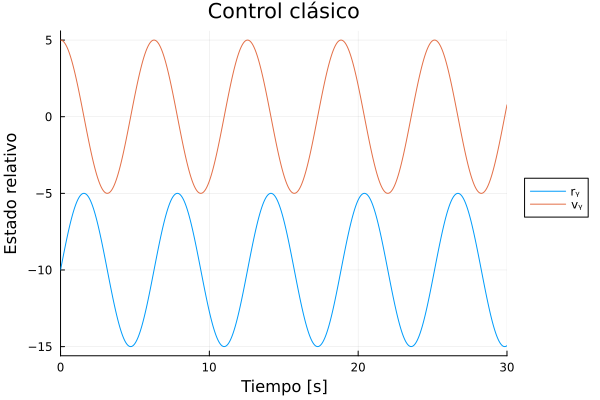
\includegraphics[width=0.76\linewidth]{lineal/estado_control_clasico.png}
  \caption{Chequeo de funcionamiento con el control de prueba $u(t)=5\sin(t)$.}
  \label{fig:lineal-prueba}
\end{figure}

\begin{figure}[H]
  \centering
  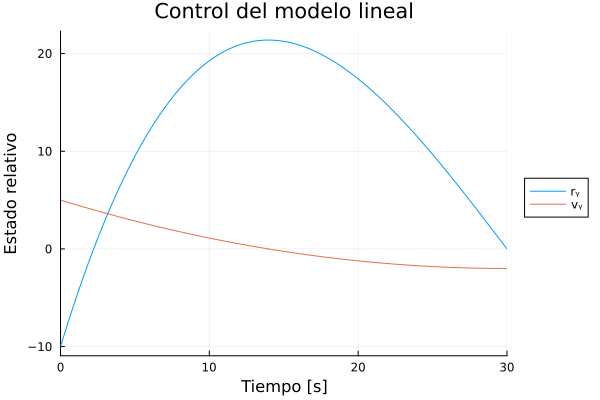
\includegraphics[width=0.76\linewidth]{lineal/estado_control_paper.png}
  \caption{Estado relativo bajo la ley del modelo lineal con restricción dura.}
  \label{fig:lineal-dura}
\end{figure}

\begin{figure}[H]
  \centering
  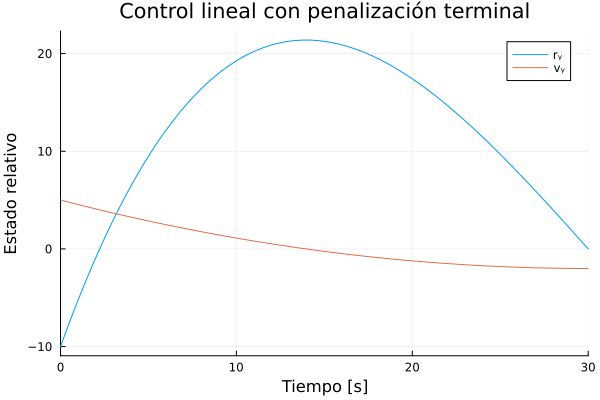
\includegraphics[width=0.76\linewidth]{lineal/estado_control_paper_margen.png}
  \caption{Estado relativo con penalización terminal $q_f=1$.}
  \label{fig:lineal-blanda}
\end{figure}

En las figuras~\ref{fig:lineal-dura} y~\ref{fig:lineal-blanda}, la posición relativa transversal se aproxima a cero al finalizar el intervalo. La velocidad transversal final no es nula. El control de prueba de la figura~\ref{fig:lineal-prueba} produce un comportamiento oscilatorio.

\begin{figure}[H]
  \centering
  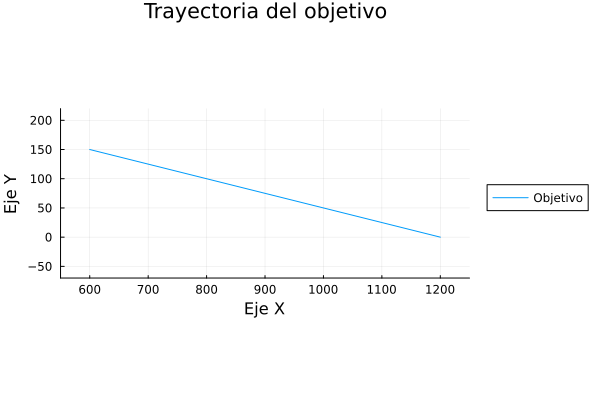
\includegraphics[width=0.76\linewidth]{lineal/trayectoria_objetivo.png}
  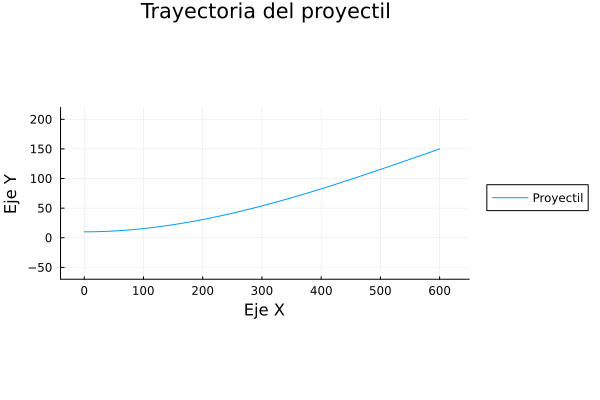
\includegraphics[width=0.76\linewidth]{lineal/trayectoria_proyectil.png}
  \caption{Trayectorias individuales del objetivo y del proyectil.}
  \label{fig:lineal-individuales}
\end{figure}

\begin{figure}[H]
  \centering
  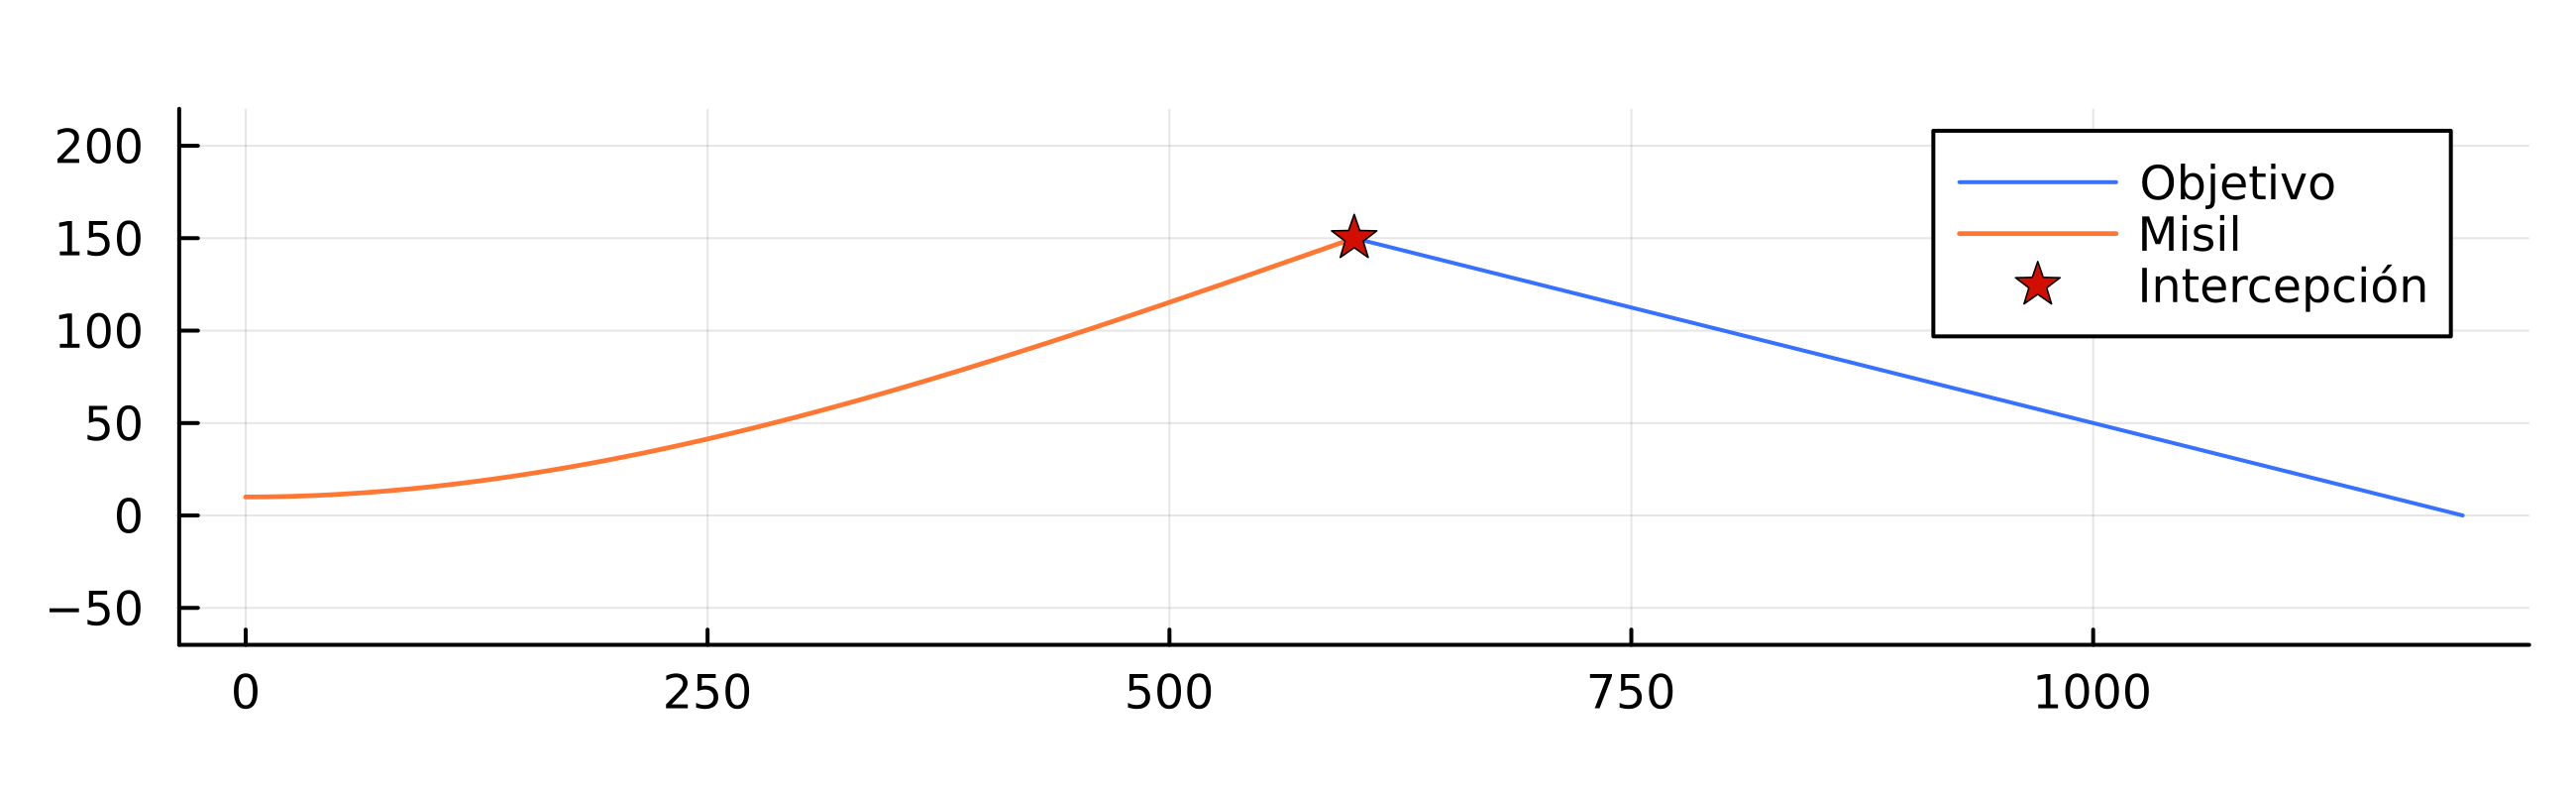
\includegraphics[width=\linewidth]{lineal/colision.png}
  % Leyenda de poster/example.tex.
  \caption{Trayectorias del objetivo y del proyectil bajo control PLC. La estrella indica la intercepción.}
  \label{fig:lineal-colision}
\end{figure}

\begin{figure}[H]
  \centering
  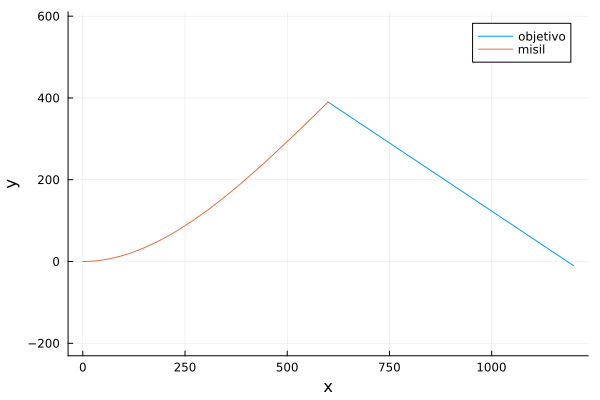
\includegraphics[width=0.76\linewidth]{lineal/lineal_colision.png}
  \caption{Gráfico adicional de trayectorias conservado en \texttt{lineal\_colision.png}. Sus condiciones de simulación no están identificadas en las salidas del notebook actual.}
  \label{fig:lineal-colision-adicional}
\end{figure}

\clearpage
\subsection{Modelo no lineal de un proyectil}
% Fuente: src/modelos/no_lineal.ipynb, celdas 3--13.
Para las simulaciones, asumimos sin pérdida de generalidad que la LOS inicial es paralela al eje $x$, pues en caso contrario basta rotar el sistema.

En \texttt{no\_lineal.ipynb}, el objetivo se ubica en $(60,0)$ y el proyectil parte desde $(0,0)$ con rapidez $V_M=5$. Se consideran los ángulos iniciales $-95^\circ$, $-90^\circ$, $-85^\circ$, $-50^\circ$ y $0^\circ$. Se utilizan $\varepsilon=0.05$, $|u|\leq5$, $t_f\leq20$, \texttt{grid\_size=50} y un máximo de 700 iteraciones. En la implementación, el denominador de la dinámica angular es $\sqrt{r_x^2+r_y^2}+10^{-4}$.

\begin{table}[H]
  \centering
  \caption{Valores registrados por Ipopt en las simulaciones no lineales. $J$ y la violación de restricciones corresponden a los valores sin escalamiento.}
  \label{tab:no-lineal}
  \small
  \begin{tabular}{@{}rrrrrrc@{}}
    \toprule
    $\alpha$ & $\beta$ & $\theta_0$ [$^\circ$] & $J$ & Violación & Iter. & Estado\\
    \midrule
    \filastabla{tablas/no_lineal.tex}
    \bottomrule
  \end{tabular}
\end{table}

Los estados de la tabla~\ref{tab:no-lineal} reproducen los mensajes del solver: O corresponde a \texttt{Optimal Solution Found}, M a \texttt{Maximum Number of Iterations Exceeded} e I a \texttt{Converged to a point of local infeasibility}. Las curvas para $-95^\circ$ y $-90^\circ$ se conservan en los gráficos, pero sus ejecuciones no registran convergencia a una solución factible. Los otros tres ángulos registran el estado O en las tres combinaciones de pesos.

Para $\theta_0=0^\circ$, las tres configuraciones muestran una trayectoria rectilínea. En los casos convergentes con $\theta_0=-85^\circ$ y $-50^\circ$, las trayectorias varían al cambiar los pesos del esfuerzo de control y del tiempo.

\begin{figure}[H]
  \centering
  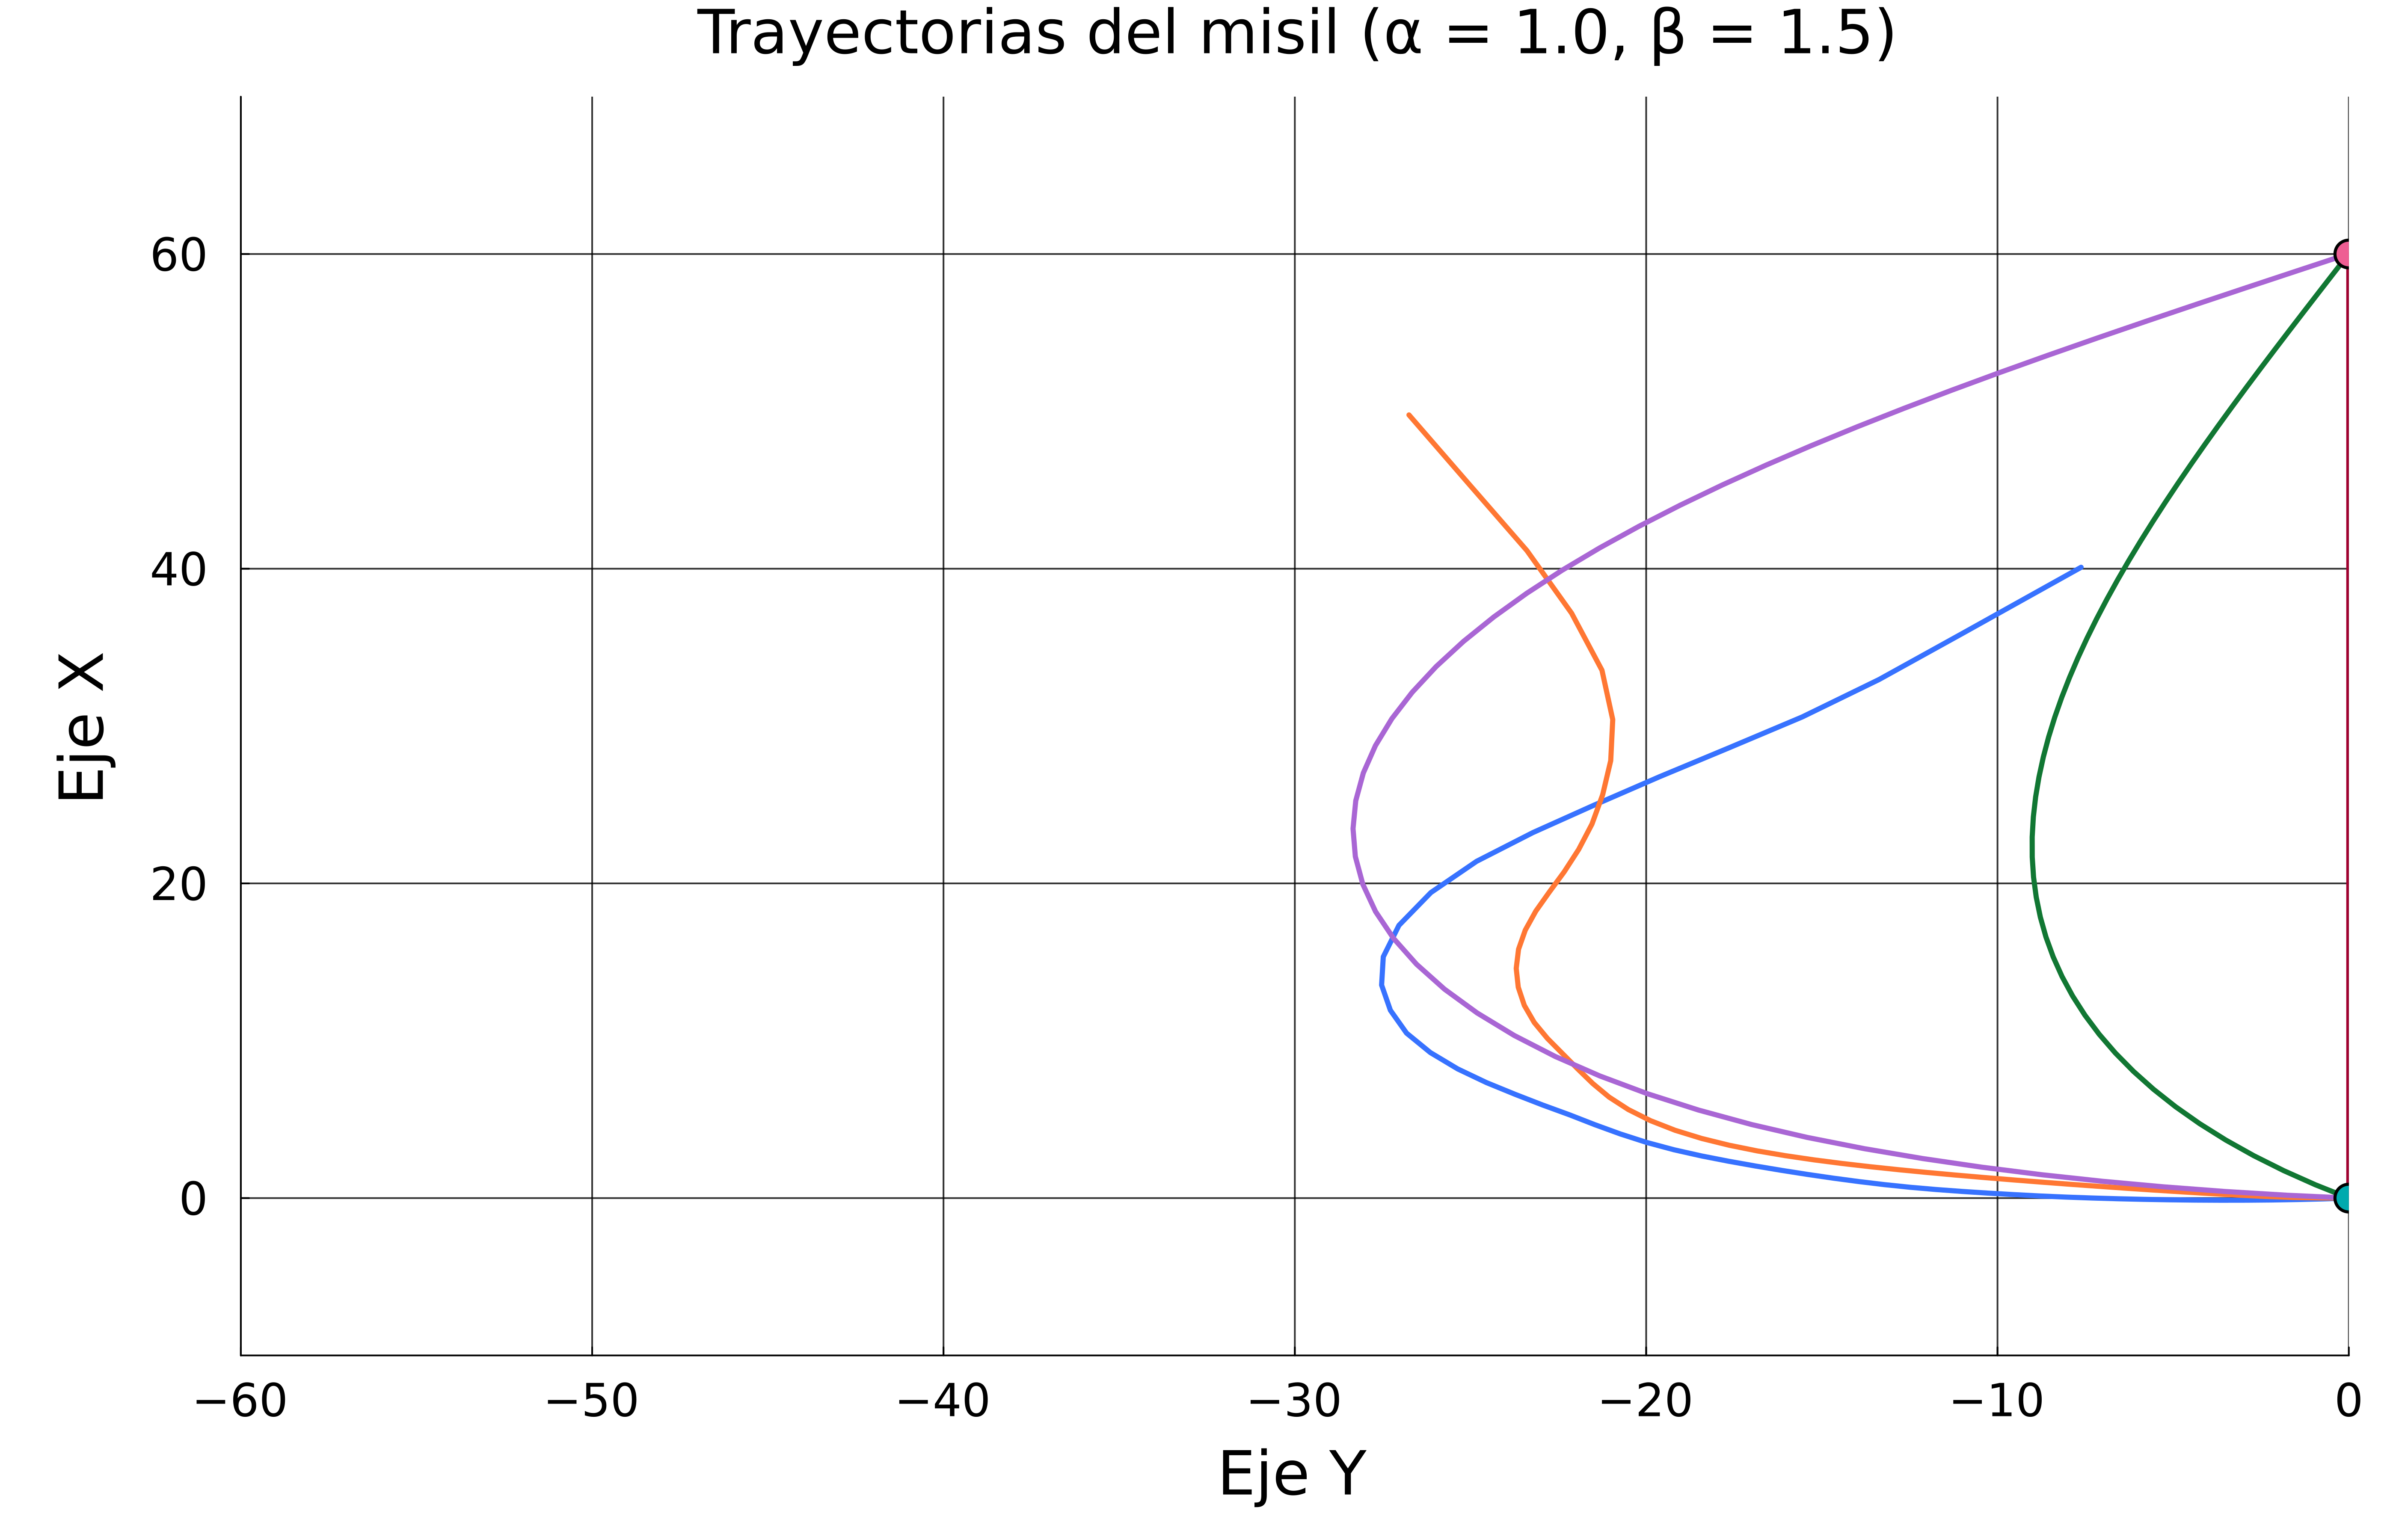
\includegraphics[width=0.9\linewidth]{no_lineal/trayectorias_alpha_1.0_beta_1.5.png}
  \caption{Trayectorias guardadas para $\alpha=1$ y $\beta=1.5$. Los estados de las cinco ejecuciones se indican en la tabla~\ref{tab:no-lineal}.}
  \label{fig:no-lineal-base}
\end{figure}

\begin{figure}[H]
  \centering
  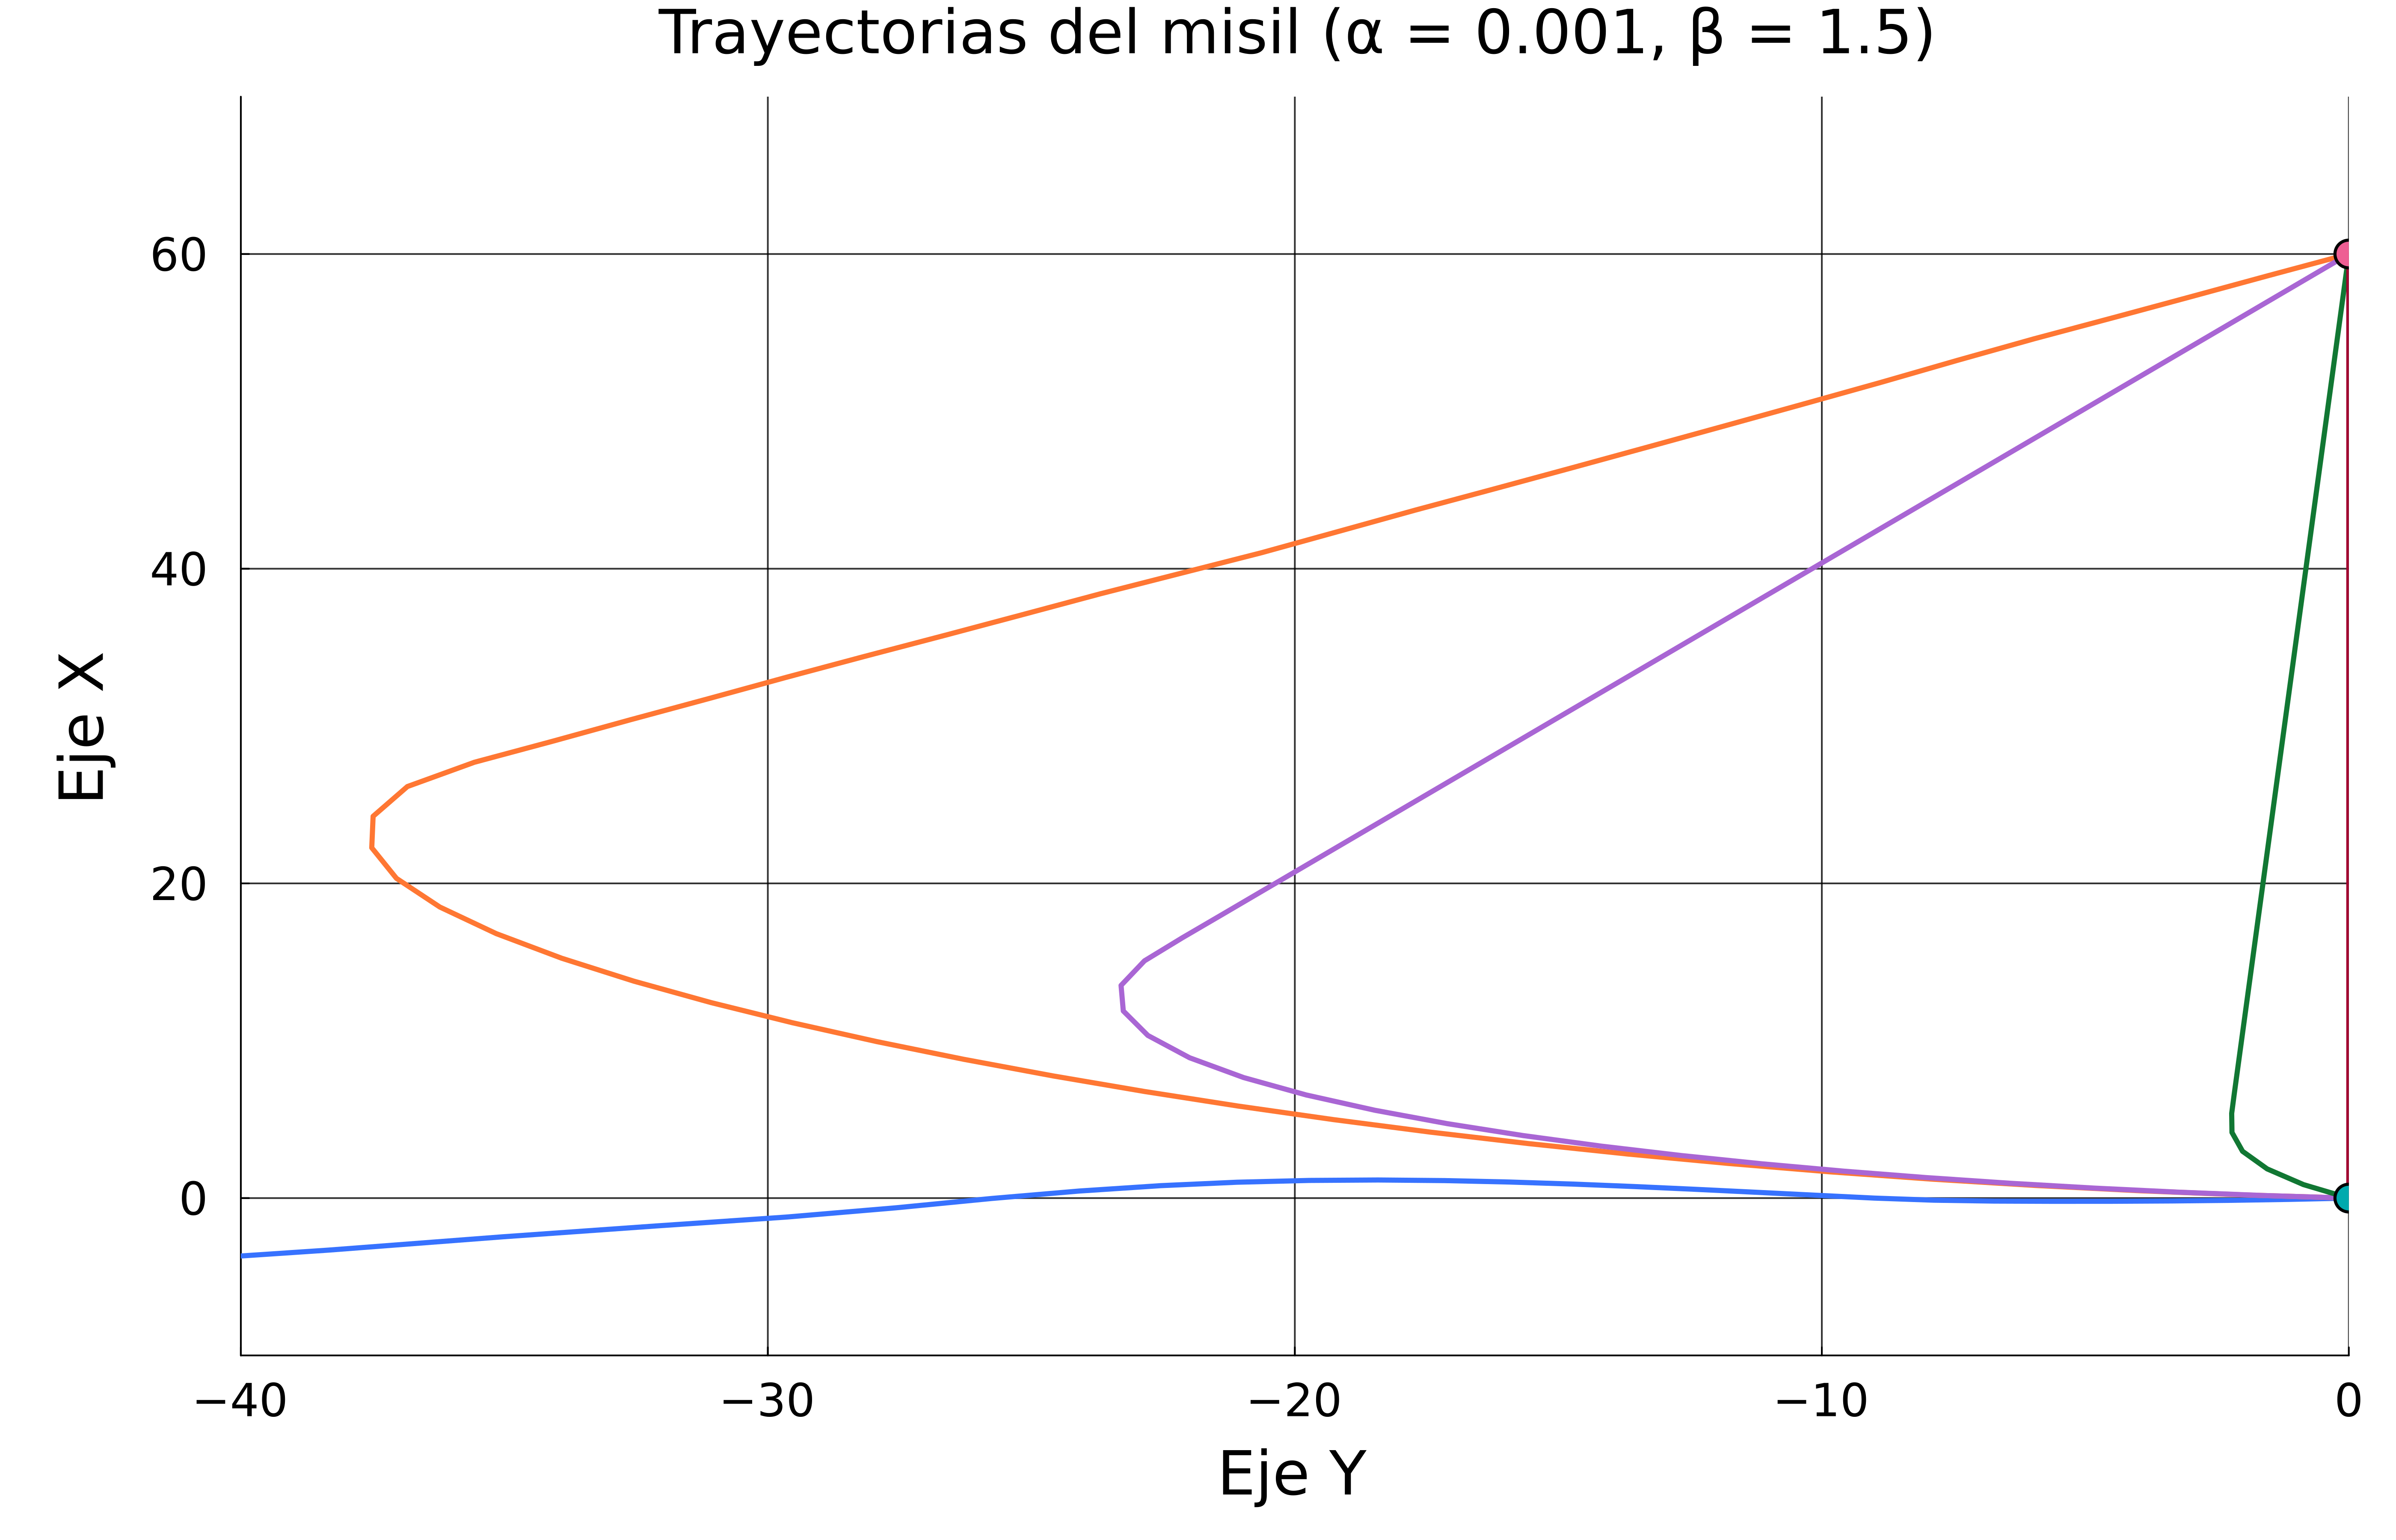
\includegraphics[width=0.9\linewidth]{no_lineal/trayectorias_alpha_0.001_beta_1.5.png}
  \caption{Trayectorias guardadas para $\alpha=0.001$ y $\beta=1.5$.}
  \label{fig:no-lineal-alpha}
\end{figure}

\begin{figure}[H]
  \centering
  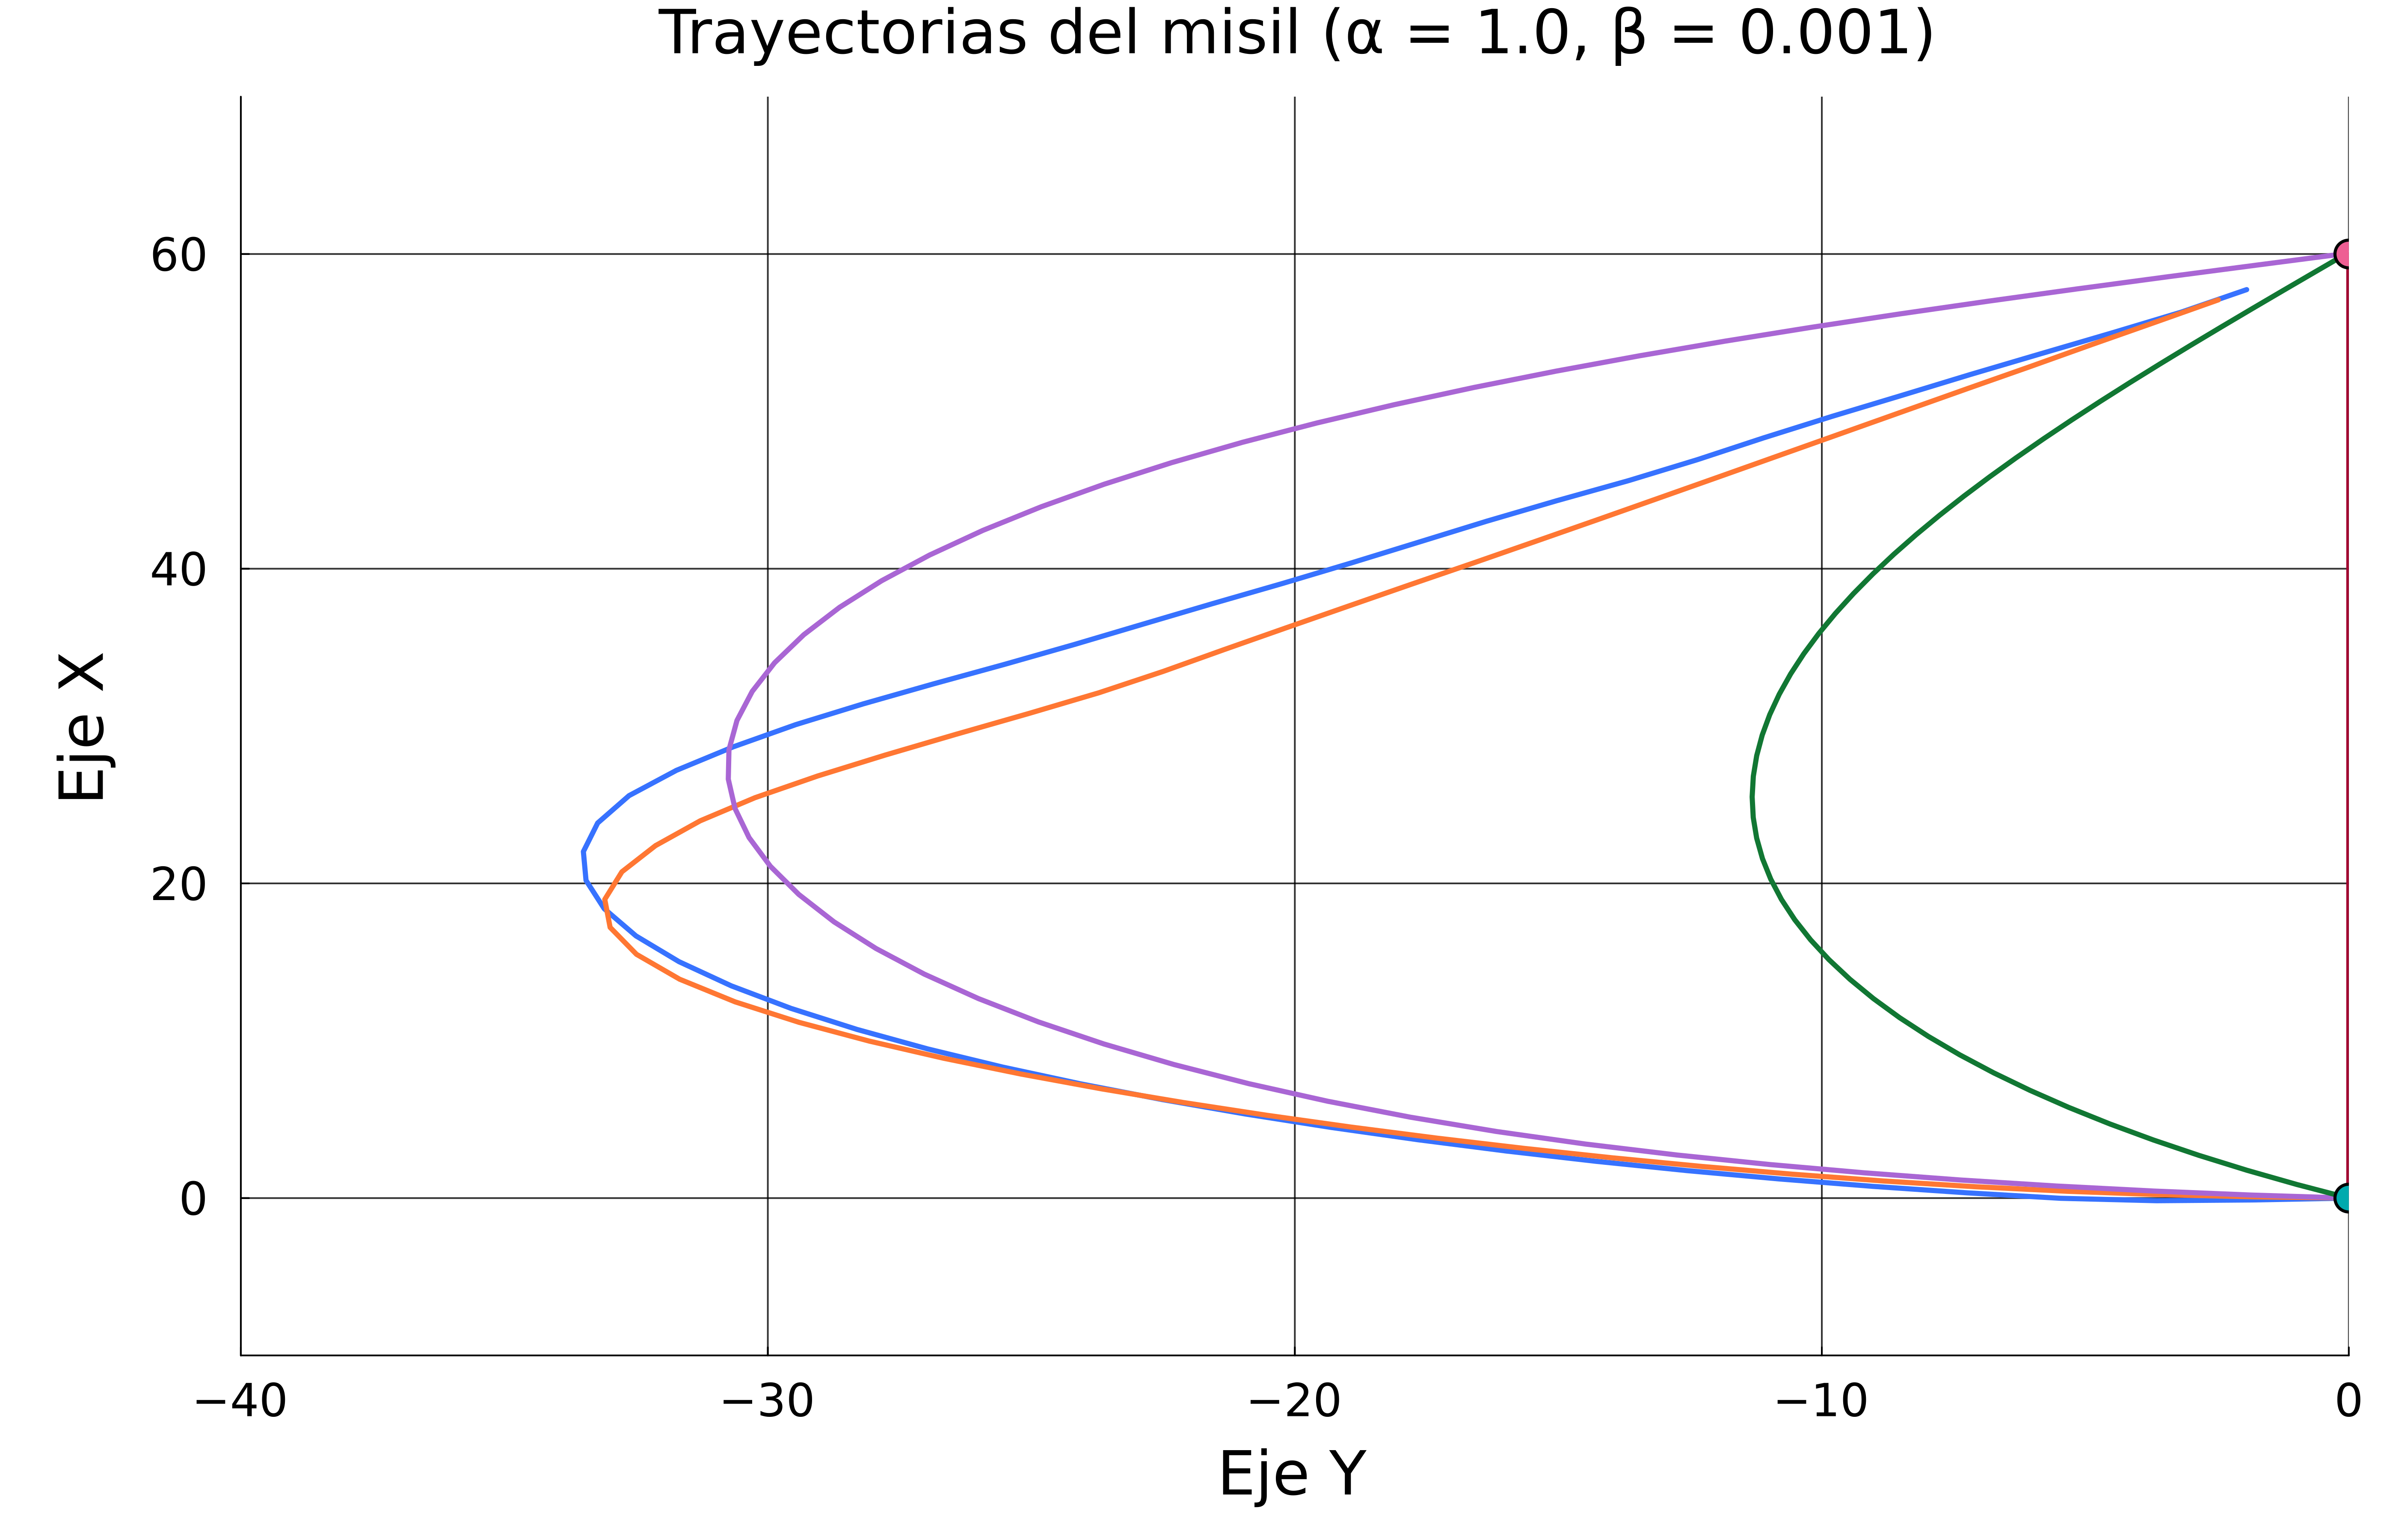
\includegraphics[width=0.9\linewidth]{no_lineal/trayectorias_alpha_1.0_beta_0.001.png}
  \caption{Trayectorias guardadas para $\alpha=1$ y $\beta=0.001$. En las tres figuras individuales, azul corresponde a $-95^\circ$, naranja a $-90^\circ$, violeta a $-85^\circ$, verde a $-50^\circ$ y rojo a $0^\circ$.}
  \label{fig:no-lineal-beta}
\end{figure}

\begin{figure}[H]
  \centering
  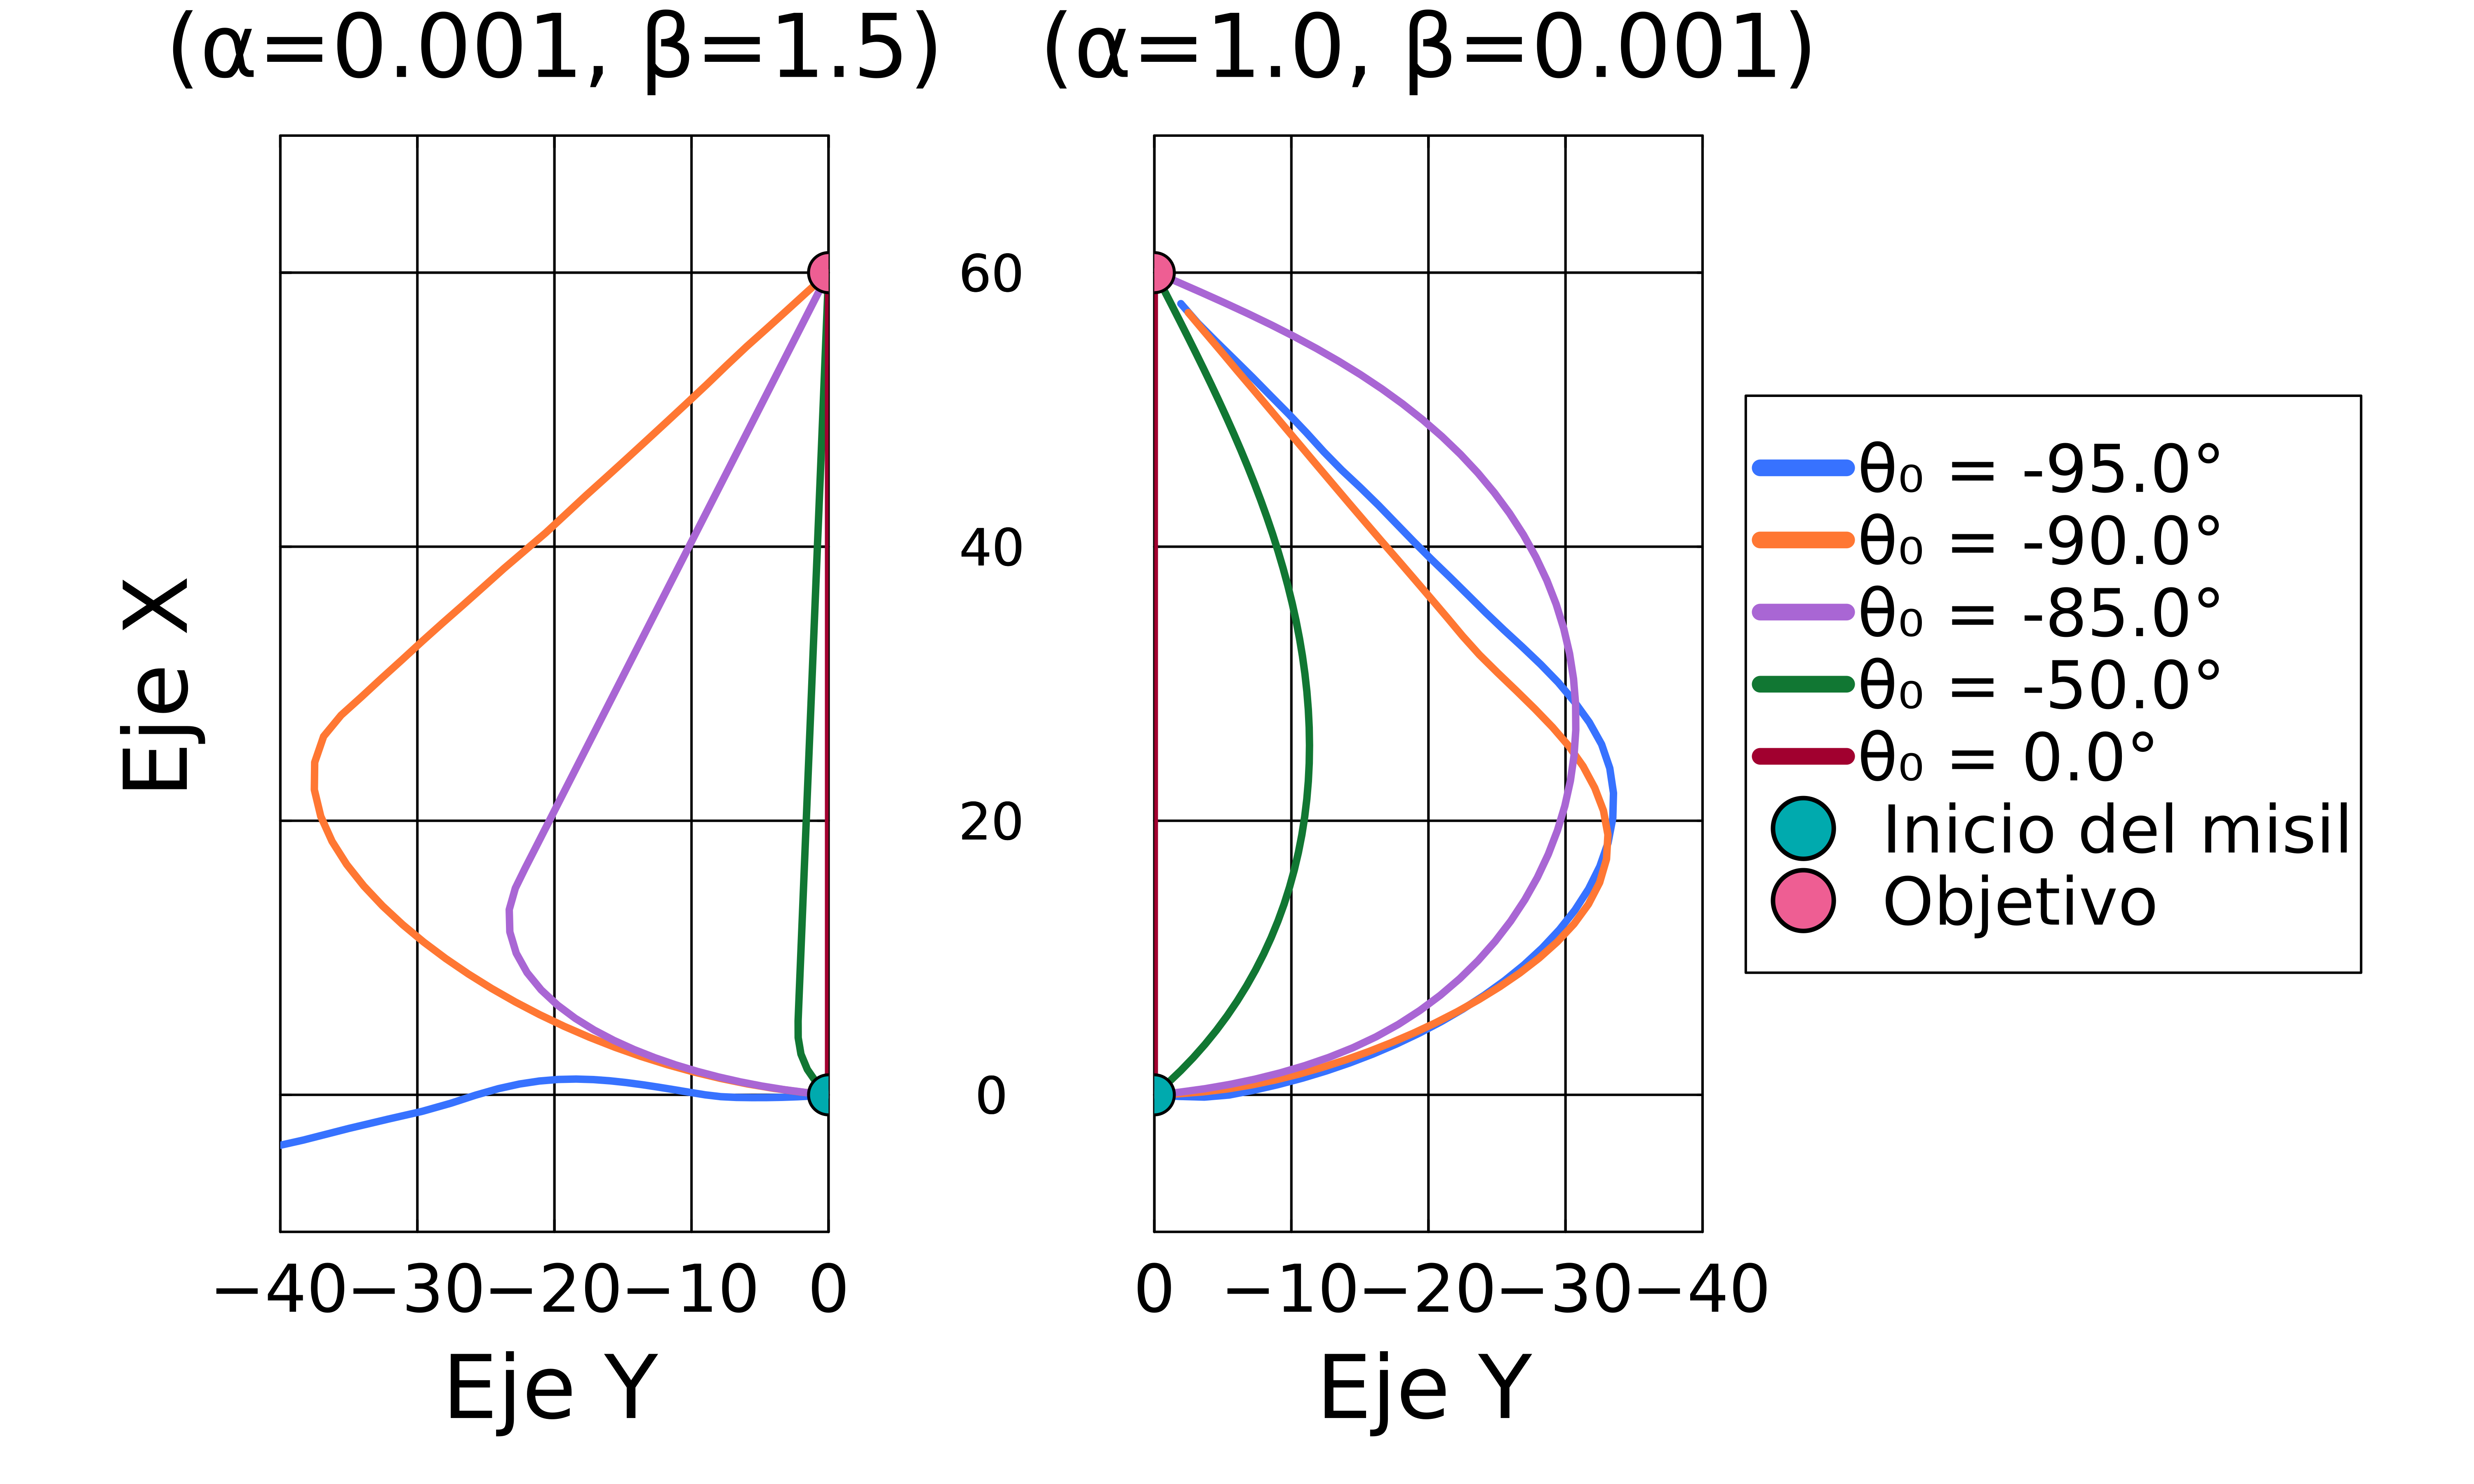
\includegraphics[width=\linewidth]{no_lineal/comparacion.png}
  % Leyenda de poster/example.tex, con los estados documentados en la tabla.
  \caption{Soluciones numéricas comparadas para distintos ángulos iniciales (panel derecho reflejado). Las curvas azul y naranja corresponden a ejecuciones sin convergencia a una solución factible.}
  \label{fig:no-lineal-comparacion}
\end{figure}

\clearpage
\subsection{Dos proyectiles acoplados}
% Fuente: src/modelos/lineal_dos_proyectiles.ipynb, celdas 3--9.
En \texttt{lineal\_dos\_proyectiles.ipynb} se comparan la simulación de la ley analítica y la discretización directa con \texttt{grid\_size=200}. Para el primer experimento se usan
$$
V_M=300,\quad t_f=10,\quad x_0=(200,-10,-250,15),\quad
\theta_d=30^\circ,\quad b=10,\quad c=100.
$$
La resolución numérica registra \texttt{Optimal Solution Found}. El costo sin escalamiento es $4514.4748191008266$ y la violación de restricciones es $2.8421709430404007\times10^{-14}$.

\begin{figure}[H]
  \centering
  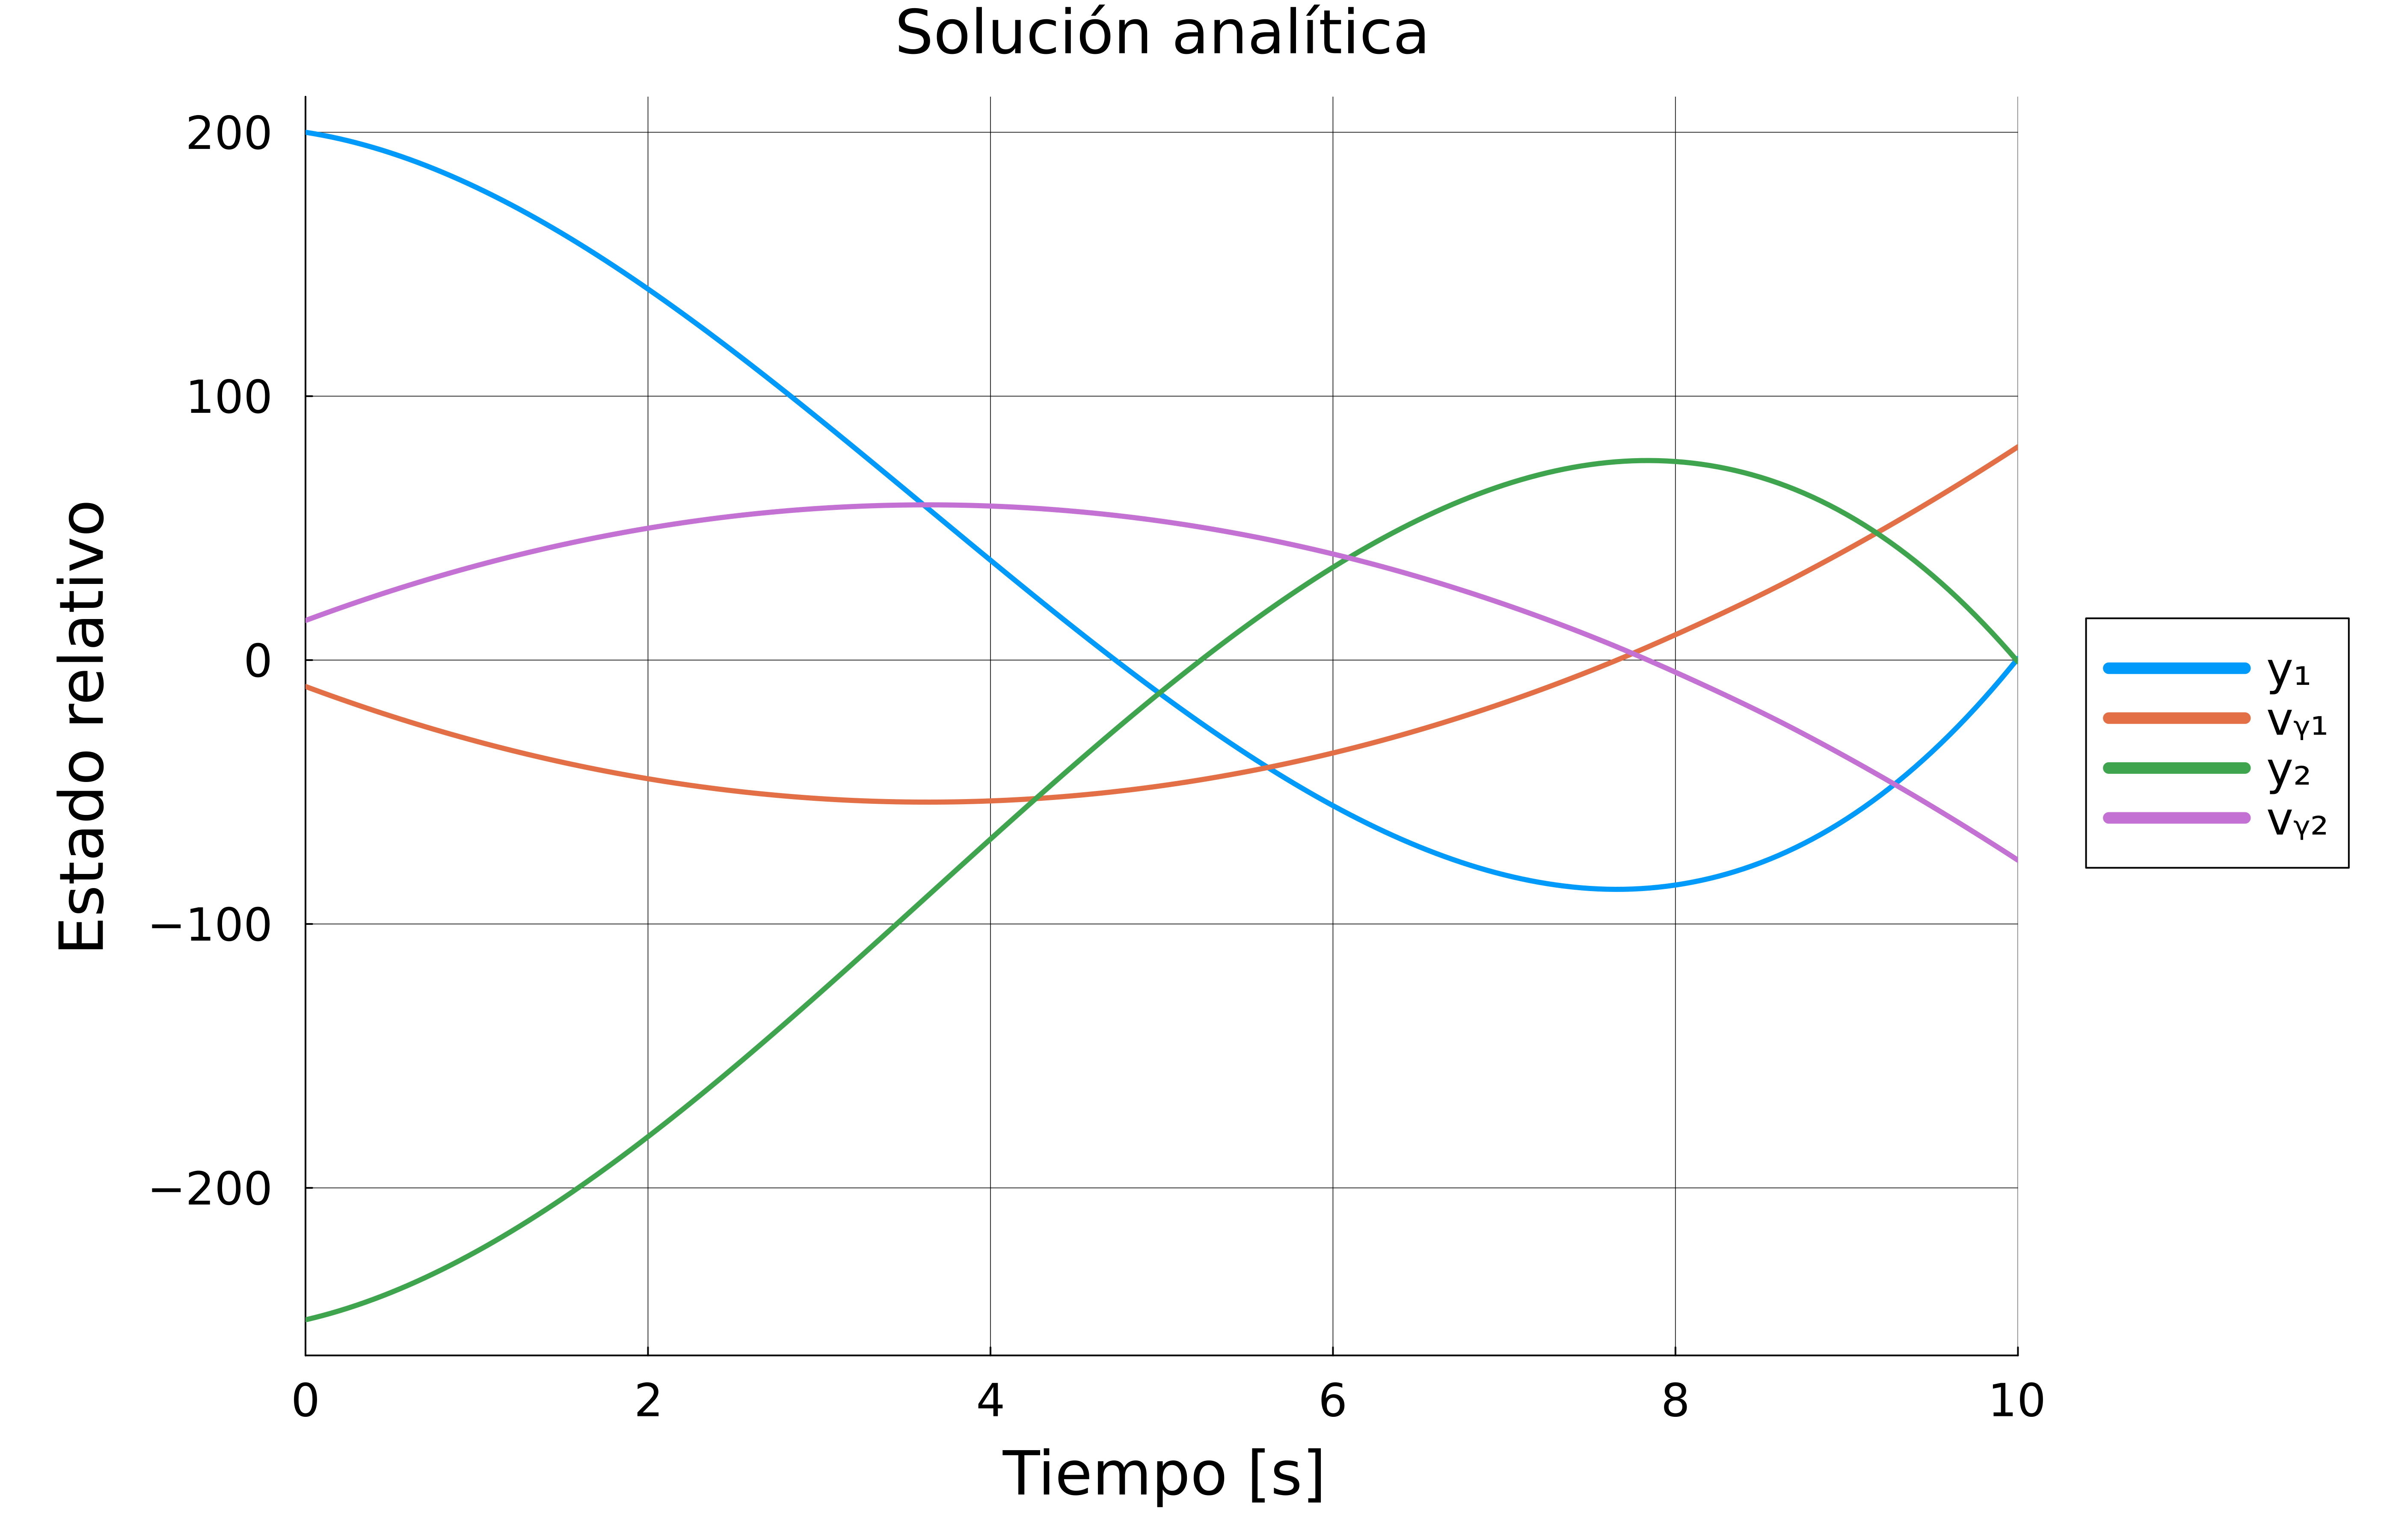
\includegraphics[width=0.95\linewidth]{lineal_dos_proyectiles/solucion_analitica.png}
  \caption{Evolución del estado bajo la ley analítica en el experimento con $\theta_d=30^\circ$.}
  \label{fig:dos-analitica}
\end{figure}

\begin{figure}[H]
  \centering
  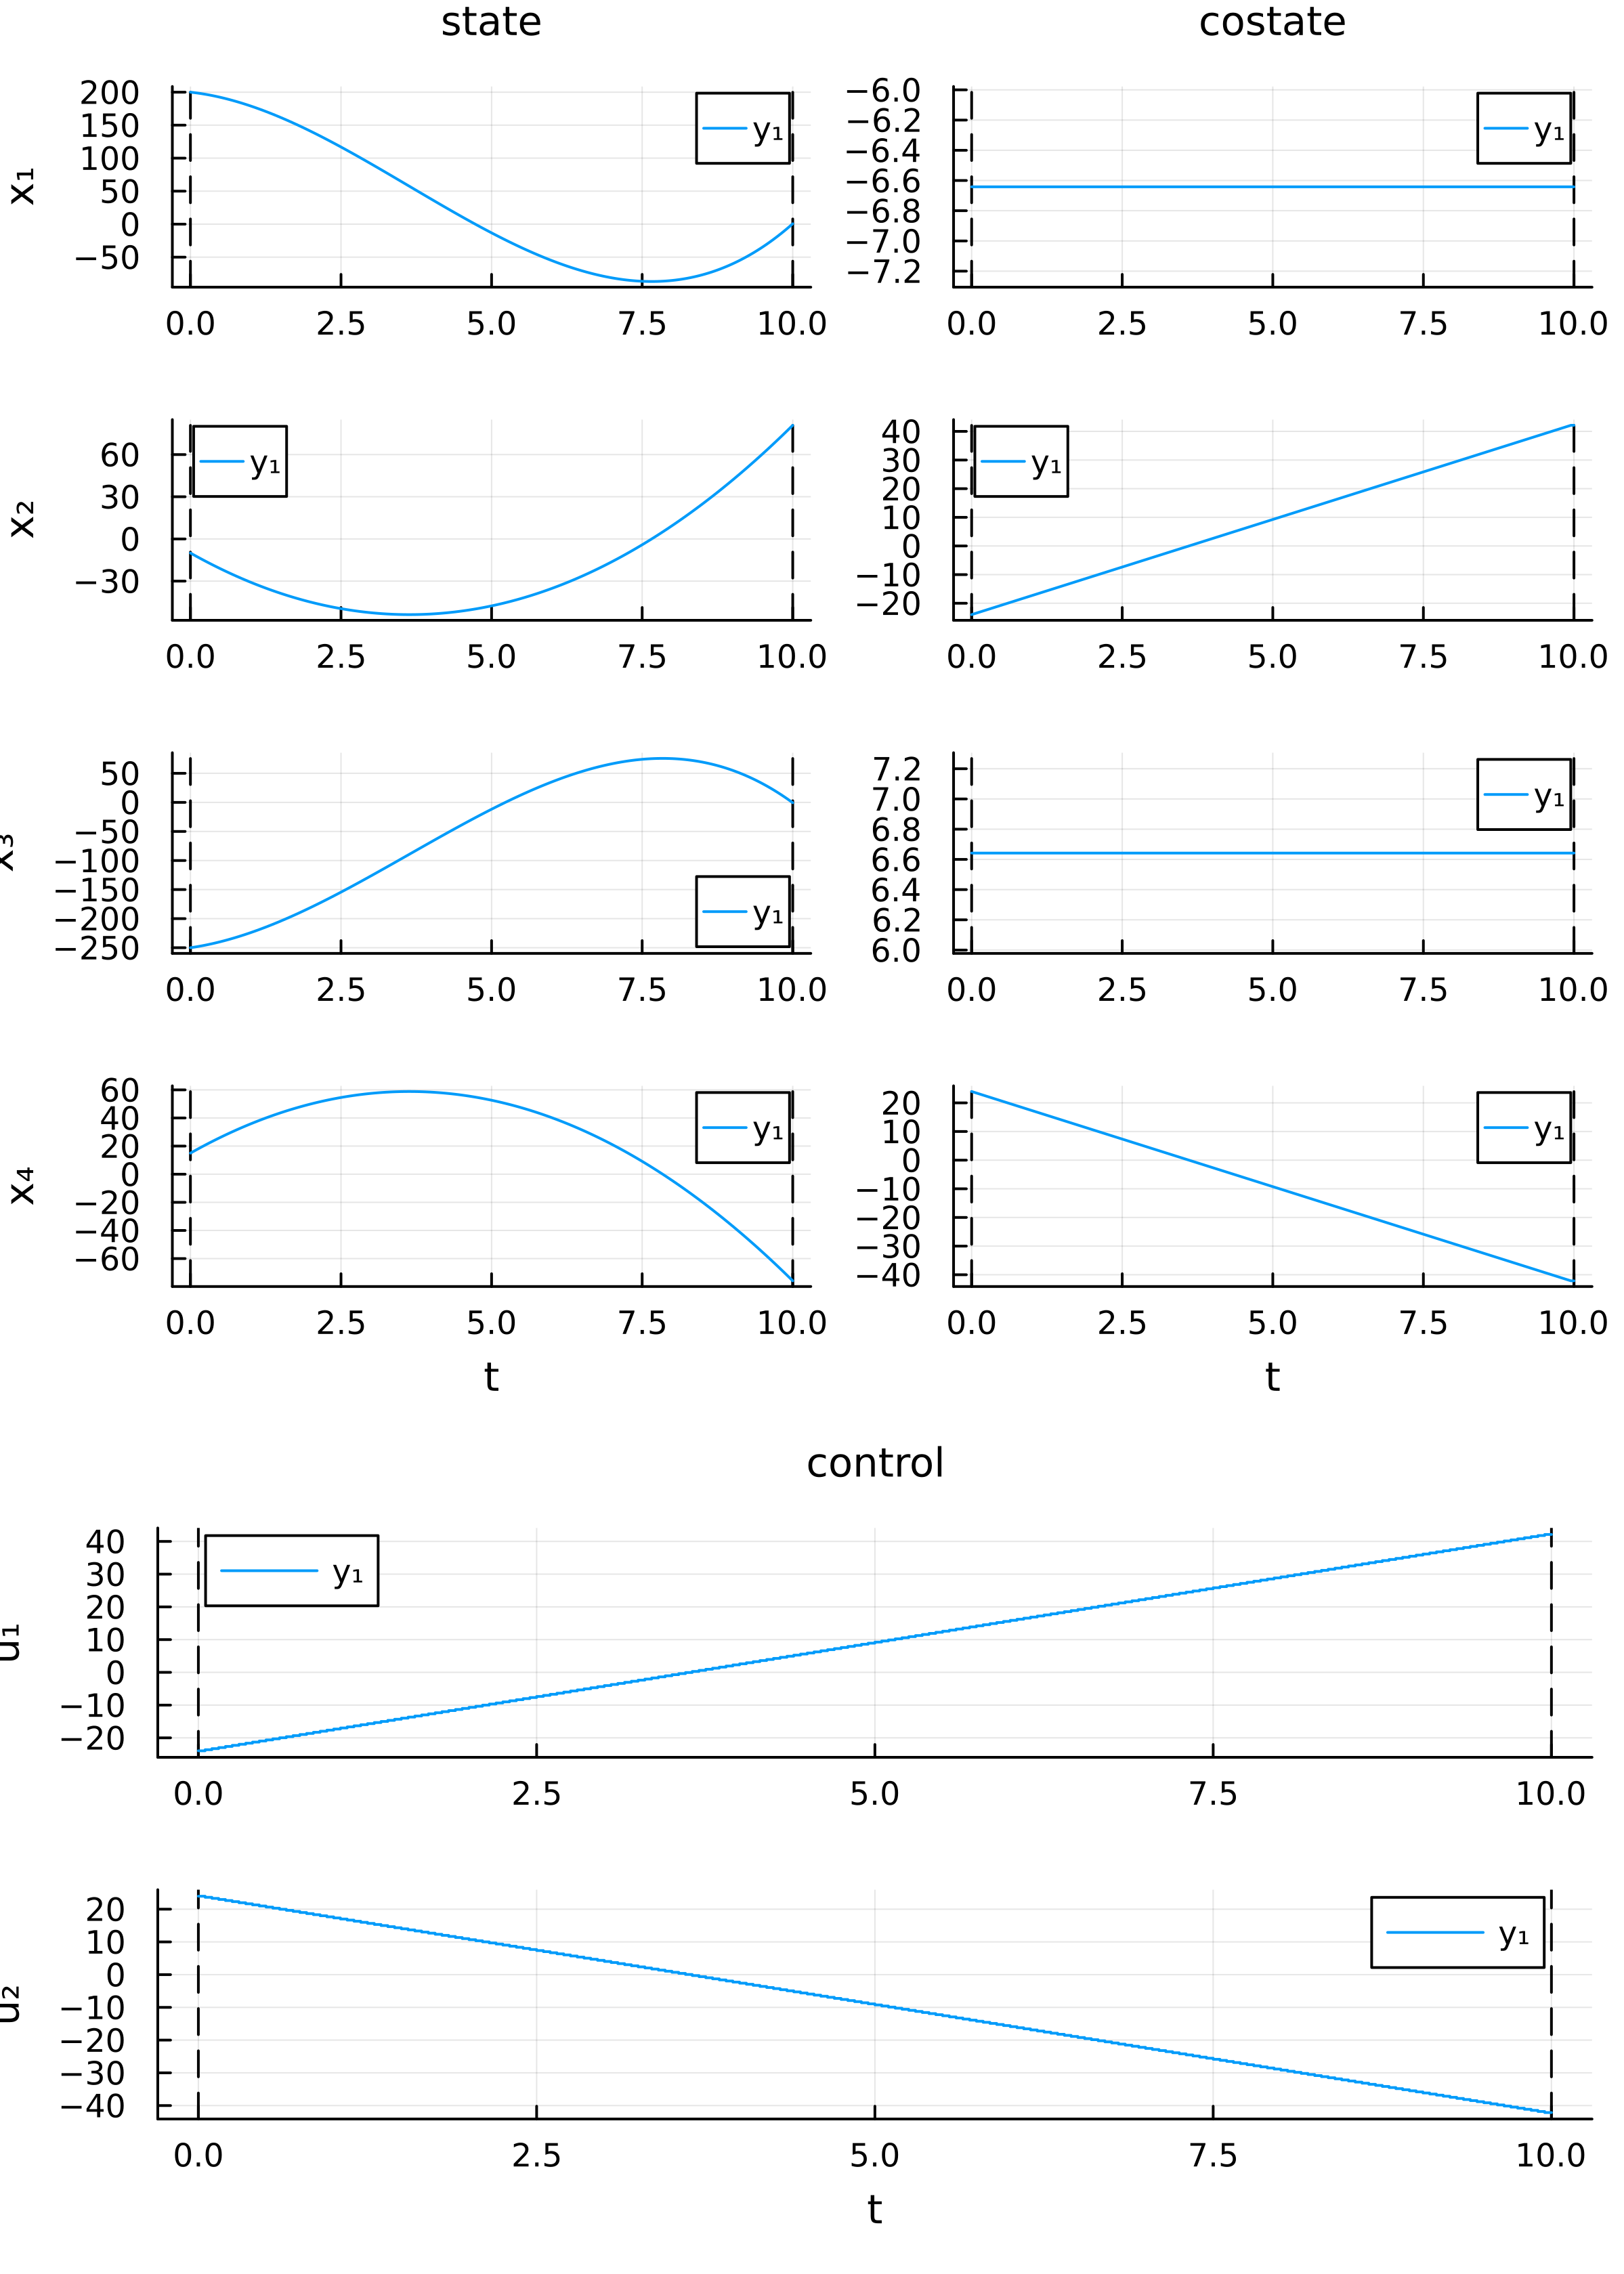
\includegraphics[width=0.93\linewidth,height=0.85\textheight,keepaspectratio]{lineal_dos_proyectiles/solucion_numerica.png}
  \caption{Estados, coestados y controles de la solución numérica para el mismo experimento.}
  \label{fig:dos-numerica}
\end{figure}

Para comparar distintos ángulos relativos de llegada, los proyectiles parten desde $(0,200)$ y $(0,-200)$, con orientación inicial $0^\circ$, y el objetivo se ubica en $(10000,200)$. Se utilizan $V_M=300$, $t_f=10000/300$, $b=1000$ y $c=10$.

\begin{table}[H]
  \centering
  \caption{Ángulos de llegada registrados en el notebook, en grados. La última columna reproduce la diferencia entre $\theta_d$ y $\Delta\theta$ de la solución analítica.}
  \label{tab:angulos}
  \small
  \begin{tabular}{@{}rrrrrrrr@{}}
    \toprule
    & \multicolumn{3}{c}{Analítica} & \multicolumn{3}{c}{Numérica} & Diferencia\\
    \cmidrule(lr){2-4}\cmidrule(lr){5-7}
    $\theta_d$ & $\theta_1$ & $\theta_2$ & $\Delta\theta$ & $\theta_1$ & $\theta_2$ & $\Delta\theta$ & $\theta_d-\Delta\theta$\\
    \midrule
    \filastabla{tablas/angulos.tex}
    \bottomrule
  \end{tabular}
\end{table}

% Texto de poster/example.tex.
Al estar asumiendo el \textbf{modelo lineal} para la obtención del control óptimo, la aproximación angular pierde precisión al aumentar $\theta_d$.
En los valores guardados, la diferencia respecto del ángulo deseado aumenta de $0.2^\circ$ a $45.1^\circ$. Las diferencias angulares obtenidas por los dos métodos son próximas entre sí.

\begin{table}[H]
  \centering
  \caption{Costo y violación de restricciones sin escalamiento en las cuatro resoluciones numéricas. Todas registran \texttt{Optimal Solution Found}.}
  \label{tab:dos-convergencia}
  \begin{tabular}{@{}rrr@{}}
    \toprule
    $\theta_d$ [$^\circ$] & $J$ & Violación de restricciones\\
    \midrule
    \filastabla{tablas/dos_proyectiles.tex}
    \bottomrule
  \end{tabular}
\end{table}

\begin{figure}[H]
  \centering
  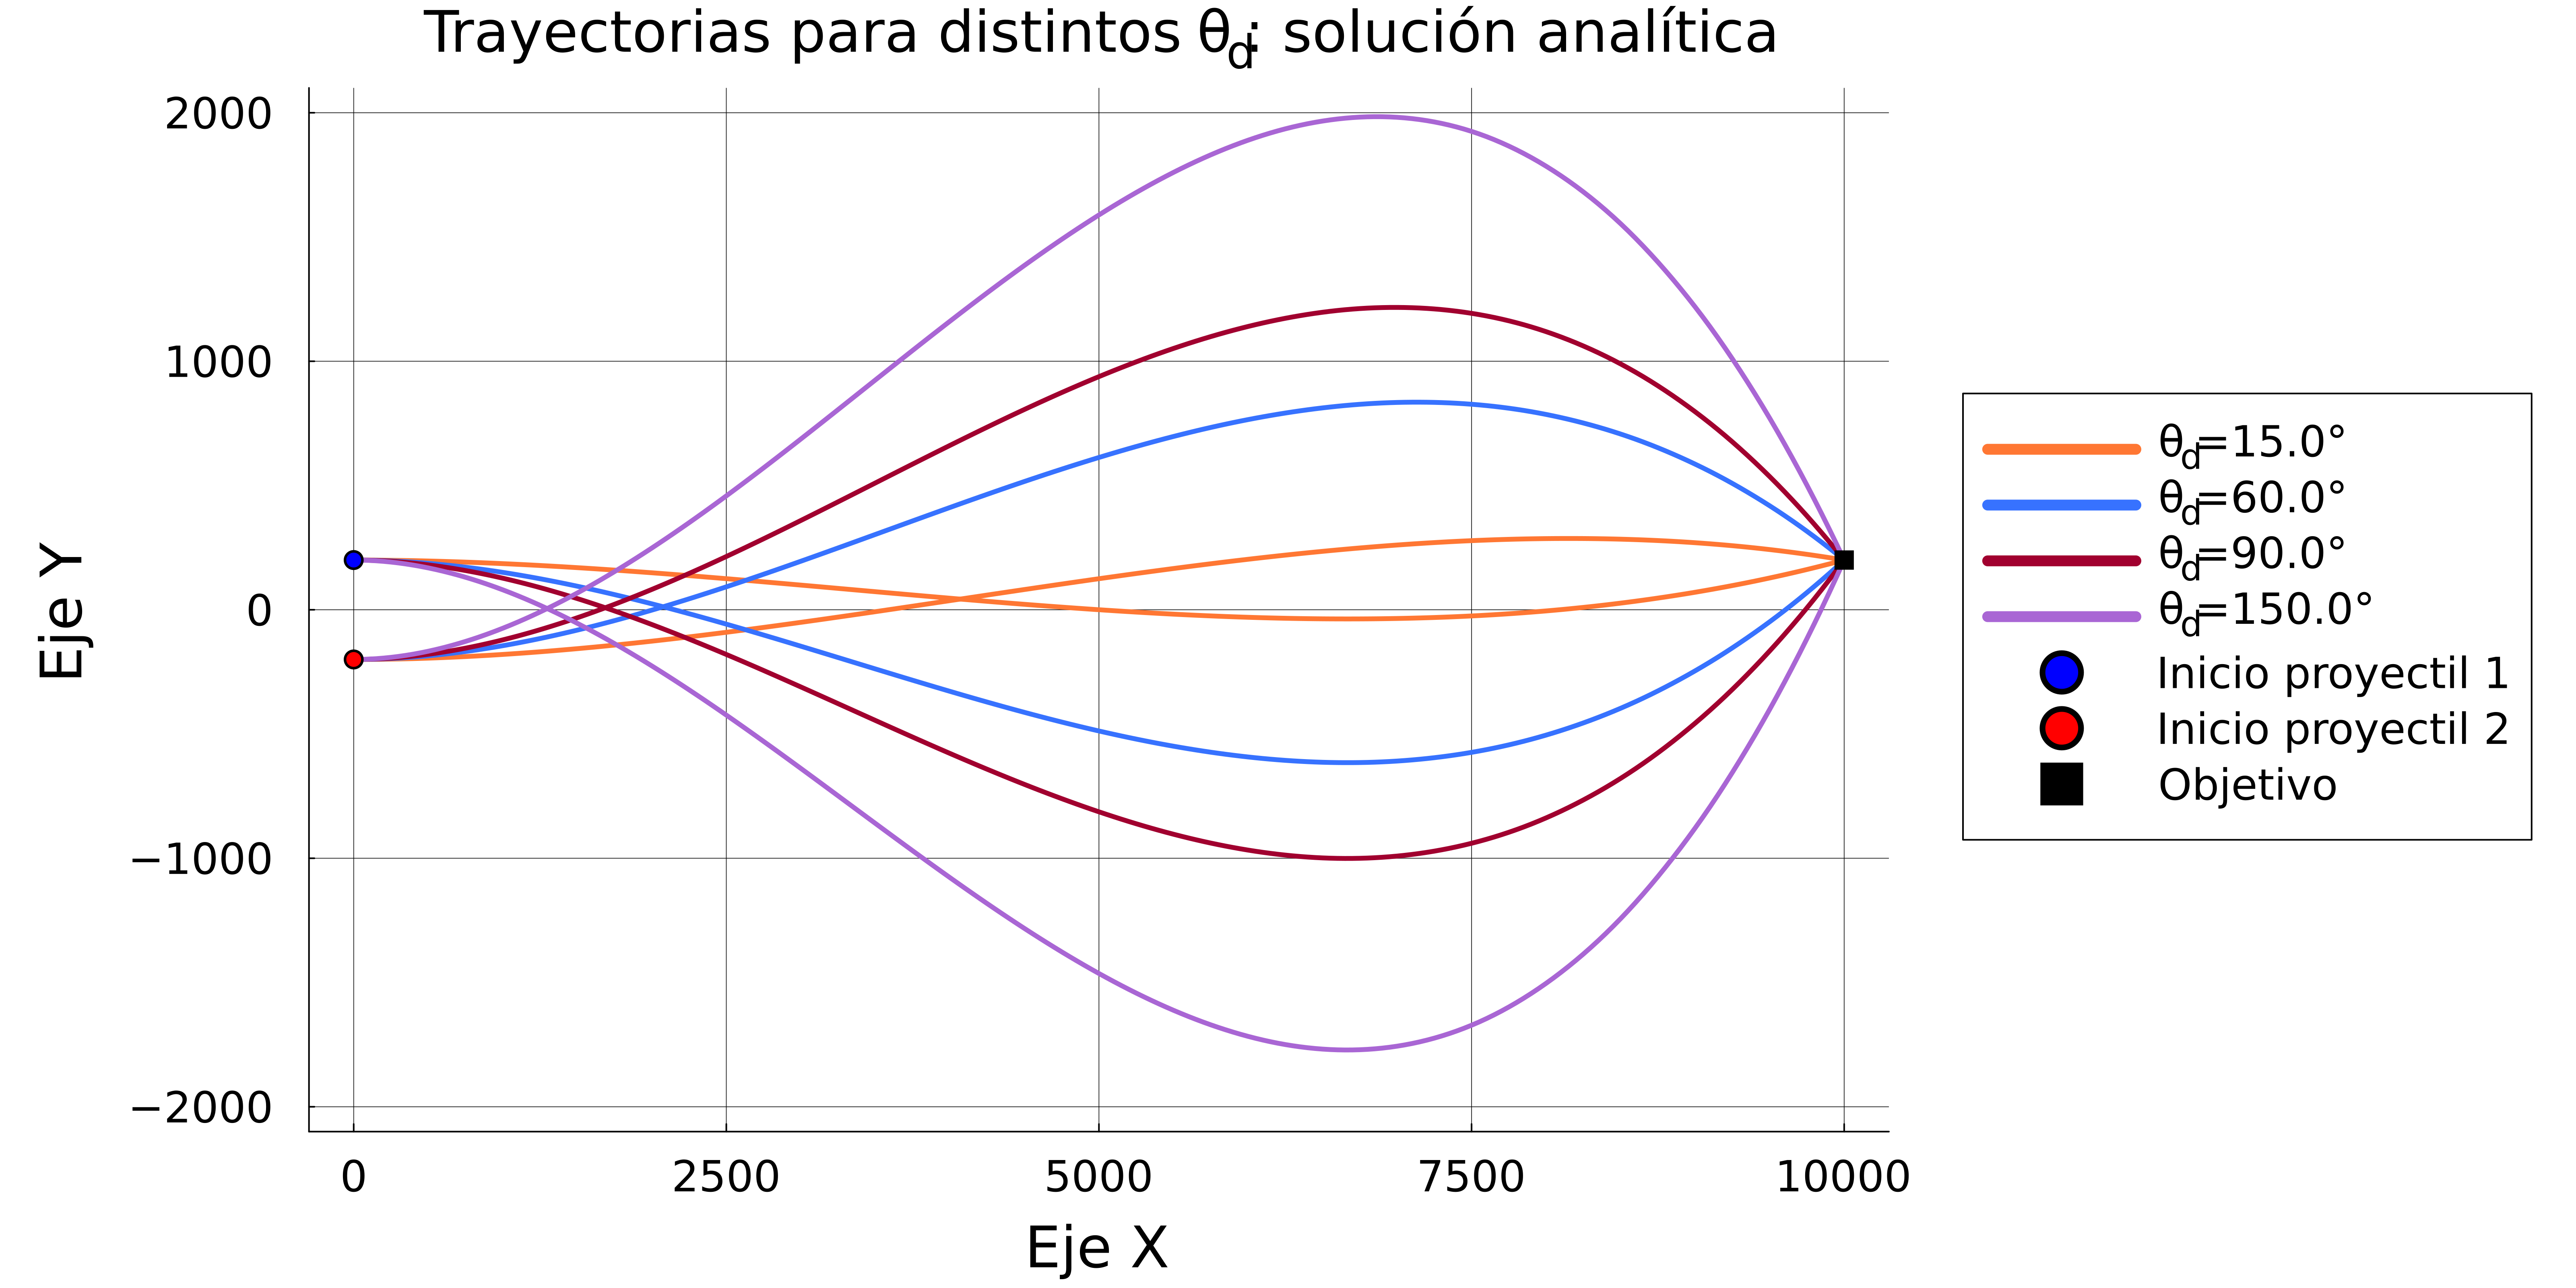
\includegraphics[width=\linewidth]{lineal_dos_proyectiles/comparacion_angulos_analitica.png}
  % Leyenda de poster/example.tex.
  \caption{Trayectorias de la solución analítica para distintos ángulos relativos deseados de llegada.}
  \label{fig:dos-angulos-analitica}
\end{figure}

\begin{figure}[H]
  \centering
  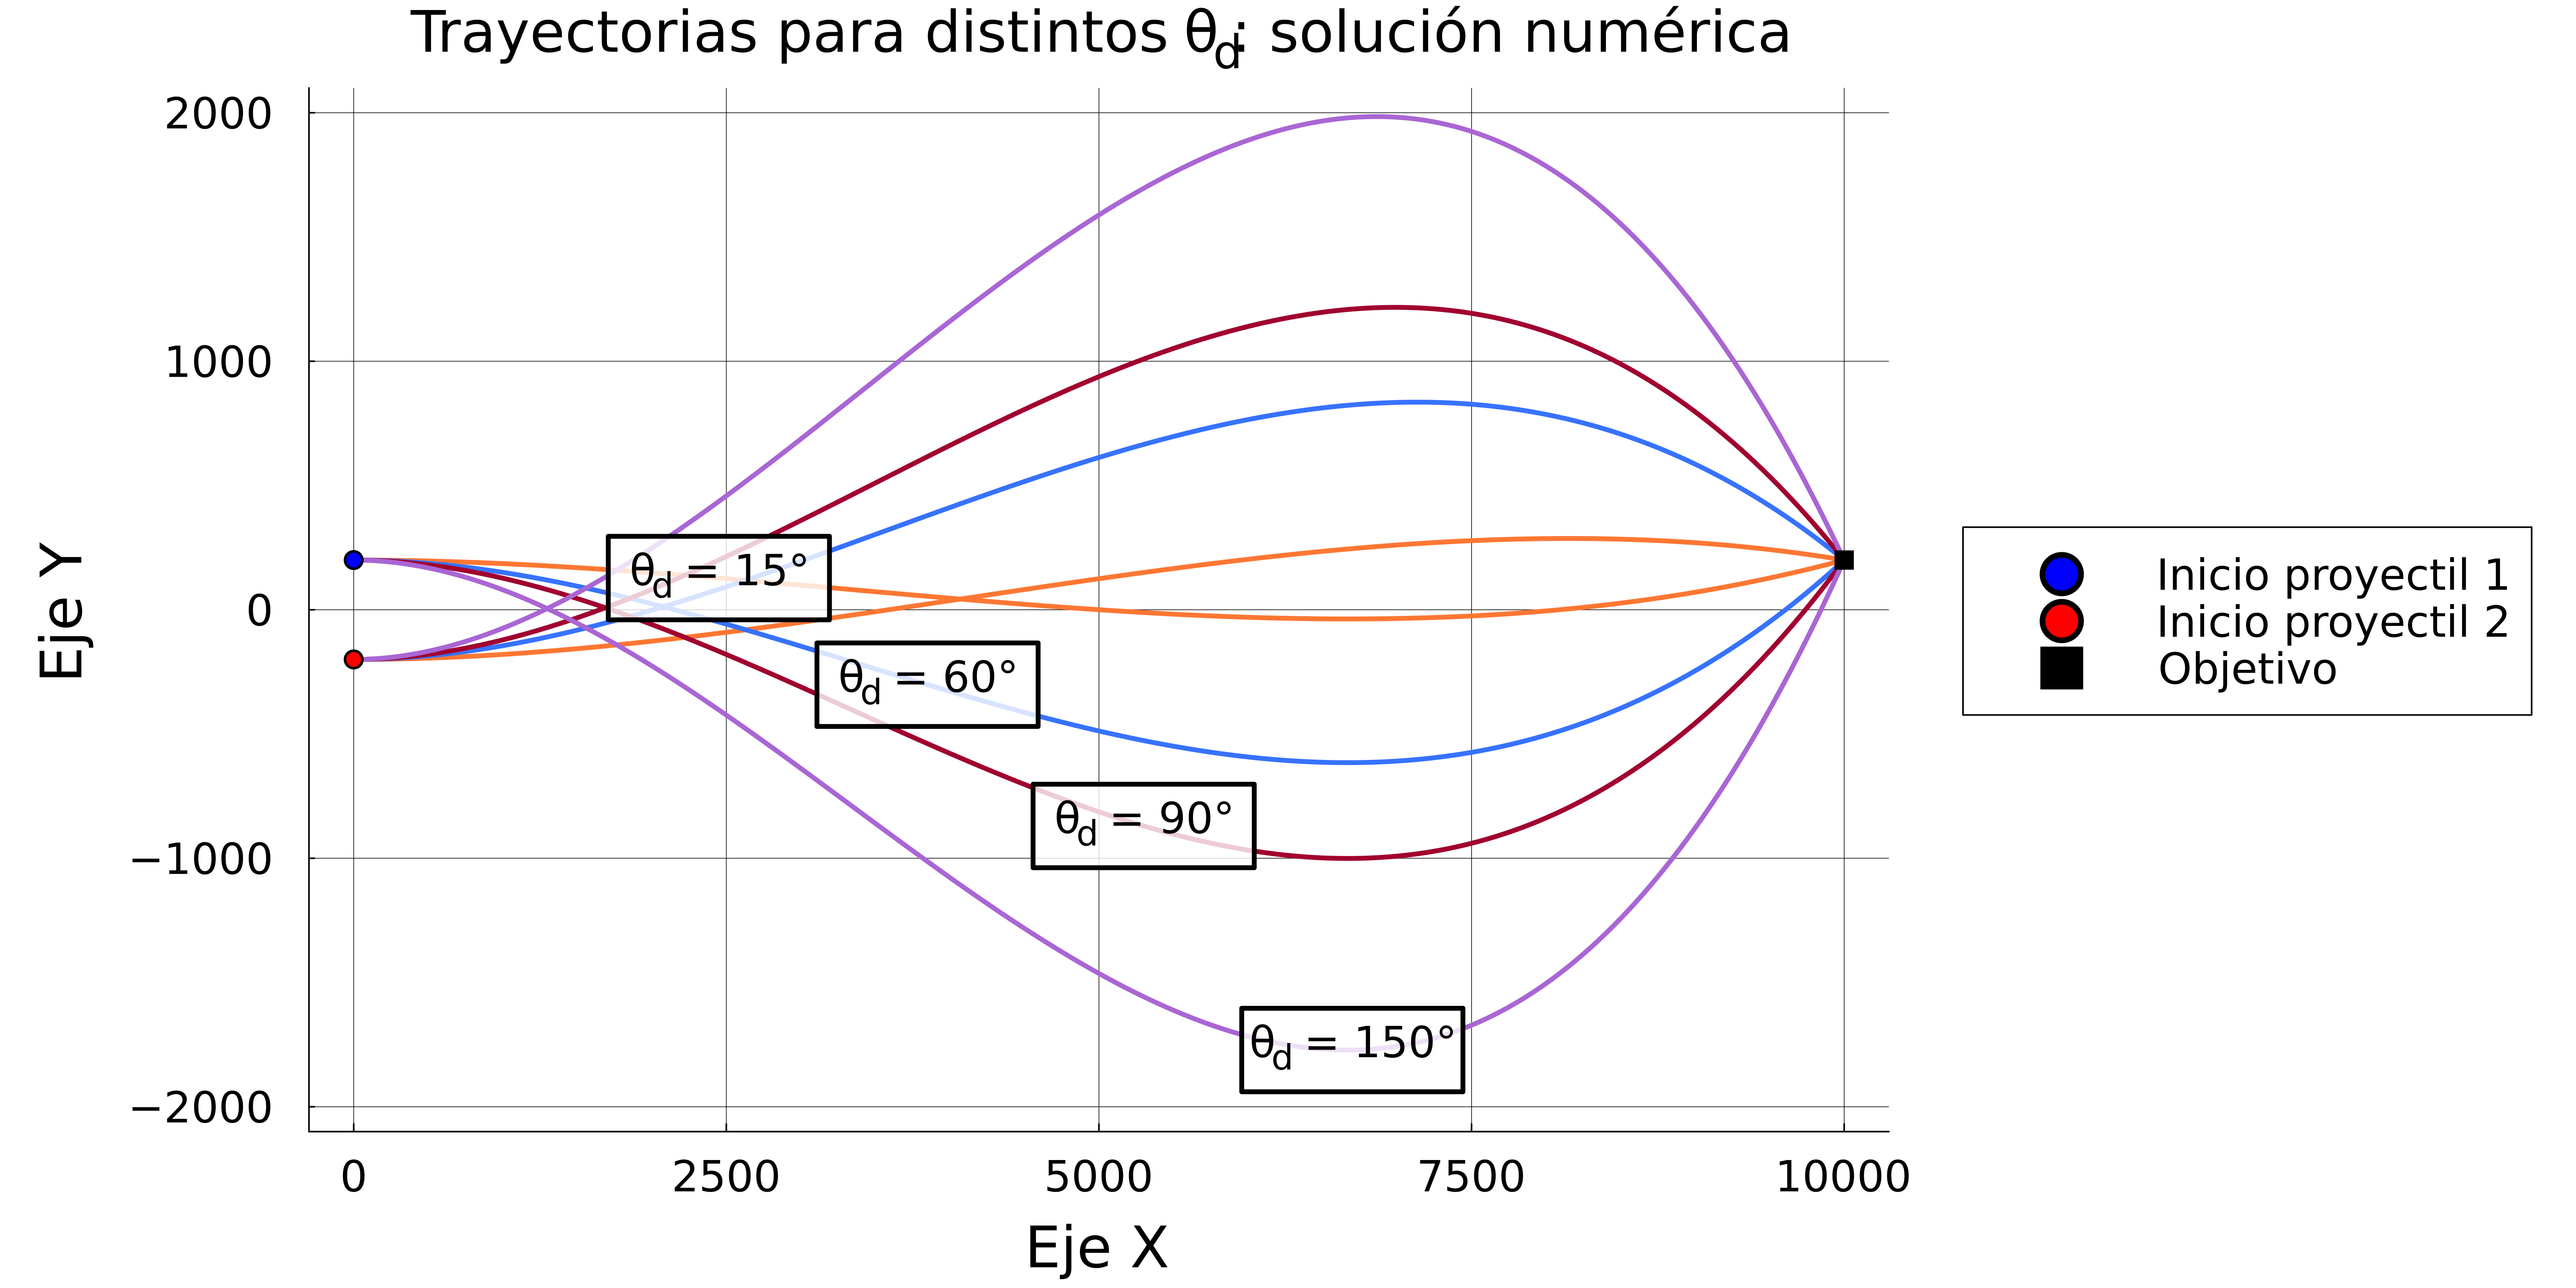
\includegraphics[width=\linewidth]{lineal_dos_proyectiles/comparacion_angulos_numerica.png}
  \caption{Trayectorias de la solución numérica para los mismos ángulos relativos deseados de llegada.}
  \label{fig:dos-angulos-numerica}
\end{figure}

\clearpage
\subsection{Modelo no lineal multiproyectil}
% Fuente: src/modelos/no_lineal_multiproyectil.ipynb, celdas 3, 5 y 9.
Los experimentos de \texttt{no\_lineal\_multiproyectil.ipynb} consideran un objetivo fijo en $(0,0)$ y rapidez $V_M=5$ para todos los proyectiles. Se utilizan $\alpha=1$, $\beta=1.5$, $\gamma=100$, $\varepsilon=0.5$, $|u_i|\leq5$ y un máximo de 6000 iteraciones. Para cada $N$ se toman las primeras $N$ filas de la tabla~\ref{tab:multi-iniciales}. La cota del tiempo final se fija en el código como
$$
t_f\leq\max\left\{35,\ 1.5\cdot1.15\,
\frac{\max_{1\leq i\leq N}\sqrt{r_{x_i}(0)^2+r_{y_i}(0)^2}}{5}\right\}.
$$

\begin{table}[H]
  \centering
  \caption{Posiciones y orientaciones iniciales de los proyectiles.}
  \label{tab:multi-iniciales}
  \begin{tabular}{@{}rrrr@{}}
    \toprule
    $i$ & $x_{M_i}(0)$ & $y_{M_i}(0)$ & $\theta_{M_i}(0)$ [$^\circ$]\\
    \midrule
    1 & 0 & -110 & 100\\
    2 & -110 & -80 & 40\\
    3 & -125 & 10 & 15\\
    4 & -80 & 105 & -40\\
    5 & 10 & 140 & -115\\
    6 & 96 & 72 & -130\\
    7 & 105 & -10 & 160\\
    8 & 75 & -100 & 115\\
    \bottomrule
  \end{tabular}
\end{table}

\begin{table}[H]
  \centering
  \caption{Estado, convergencia y violación de restricciones registrados por \texttt{status}, \texttt{successful} y \texttt{constraints\_violation}.}
  \label{tab:multi-convergencia}
  \begin{tabular}{@{}rllr@{}}
    \toprule
    $N$ & Estado & Convergencia & Violación de restricciones\\
    \midrule
    \filastabla{tablas/multiproyectil.tex}
    \bottomrule
  \end{tabular}
\end{table}

Las ocho ejecuciones registran convergencia. La mayor violación de restricciones reportada corresponde a $N=4$, con aproximadamente $1.15\times10^{-6}$. Estos registros corresponden al problema discretizado. El tiempo final común y la penalización de las holguras no constituyen una comprobación de que todas las primeras llegadas ocurran exactamente al mismo instante.

\begin{figure}[H]
  \centering
  \includegraphics[width=\linewidth]{multiproyectil/trayectorias_N1.png}
  \caption{Trayectoria de un proyectil con penalización de entrada anticipada. \href{run:figuras/multiproyectil/trayectorias_N1.gif}{Animación original}.}
  \label{fig:multi-1}
\end{figure}

\begin{figure}[H]
  \centering
  \includegraphics[width=\linewidth]{multiproyectil/trayectorias_N2.png}
  \caption{Trayectorias de 2 proyectiles con tiempo final común y penalización de llegadas anticipadas.}
  \label{fig:multi-2}
\end{figure}

\begin{figure}[H]
  \centering
  \includegraphics[width=\linewidth]{multiproyectil/trayectorias_N3.png}
  \caption{Trayectorias de 3 proyectiles con tiempo final común y penalización de llegadas anticipadas. \href{run:figuras/multiproyectil/trayectorias_N3.gif}{Animación original}.}
  \label{fig:multi-3}
\end{figure}

\begin{figure}[H]
  \centering
  \includegraphics[width=\linewidth]{multiproyectil/trayectorias_N4.png}
  \caption{Trayectorias de 4 proyectiles con tiempo final común y penalización de llegadas anticipadas. \href{run:figuras/multiproyectil/trayectorias_N4.gif}{Animación original}.}
  \label{fig:multi-4}
\end{figure}

\begin{figure}[H]
  \centering
  \includegraphics[width=\linewidth]{multiproyectil/trayectorias_N5.png}
  \caption{Trayectorias de 5 proyectiles con tiempo final común y penalización de llegadas anticipadas. \href{run:figuras/multiproyectil/trayectorias_N5.gif}{Animación original}.}
  \label{fig:multi-5}
\end{figure}

\begin{figure}[H]
  \centering
  \includegraphics[width=\linewidth]{multiproyectil/trayectorias_N6.png}
  \caption{Trayectorias de 6 proyectiles con tiempo final común y penalización de llegadas anticipadas. \href{run:figuras/multiproyectil/trayectorias_N6.gif}{Animación original}.}
  \label{fig:multi-6}
\end{figure}

\begin{figure}[H]
  \centering
  \includegraphics[width=\linewidth]{multiproyectil/trayectorias_N7.png}
  \caption{Trayectorias de 7 proyectiles con tiempo final común y penalización de llegadas anticipadas. \href{run:figuras/multiproyectil/trayectorias_N7.gif}{Animación original}.}
  \label{fig:multi-7}
\end{figure}

\begin{figure}[H]
  \centering
  \includegraphics[width=\linewidth]{multiproyectil/trayectorias_N8.png}
  \caption{Trayectorias de 8 proyectiles con tiempo final común y penalización de llegadas anticipadas. \href{run:figuras/multiproyectil/trayectorias_N8.gif}{Animación original}.}
  \label{fig:multi-8}
\end{figure}


\subsubsection{Dos proyectiles con distancias iniciales diferentes}
% Fuente: última celda de src/modelos/no_lineal_multiproyectil.ipynb y GIF existentes.
El segundo experimento utiliza posiciones iniciales $(-10,0)$ y $(150,0)$, orientaciones $45^\circ$ y $225^\circ$, rapidez $V_M=2$ y pesos $\gamma=100$ y $\gamma=0.0001$. El código fija $t_f\leq(150/2)\cdot1.15\cdot1.5$. Se conservan las dos animaciones, pero la celda no contiene salidas de estado del solver ni valores de violación de restricciones.

\begin{figure}[H]
  \centering
  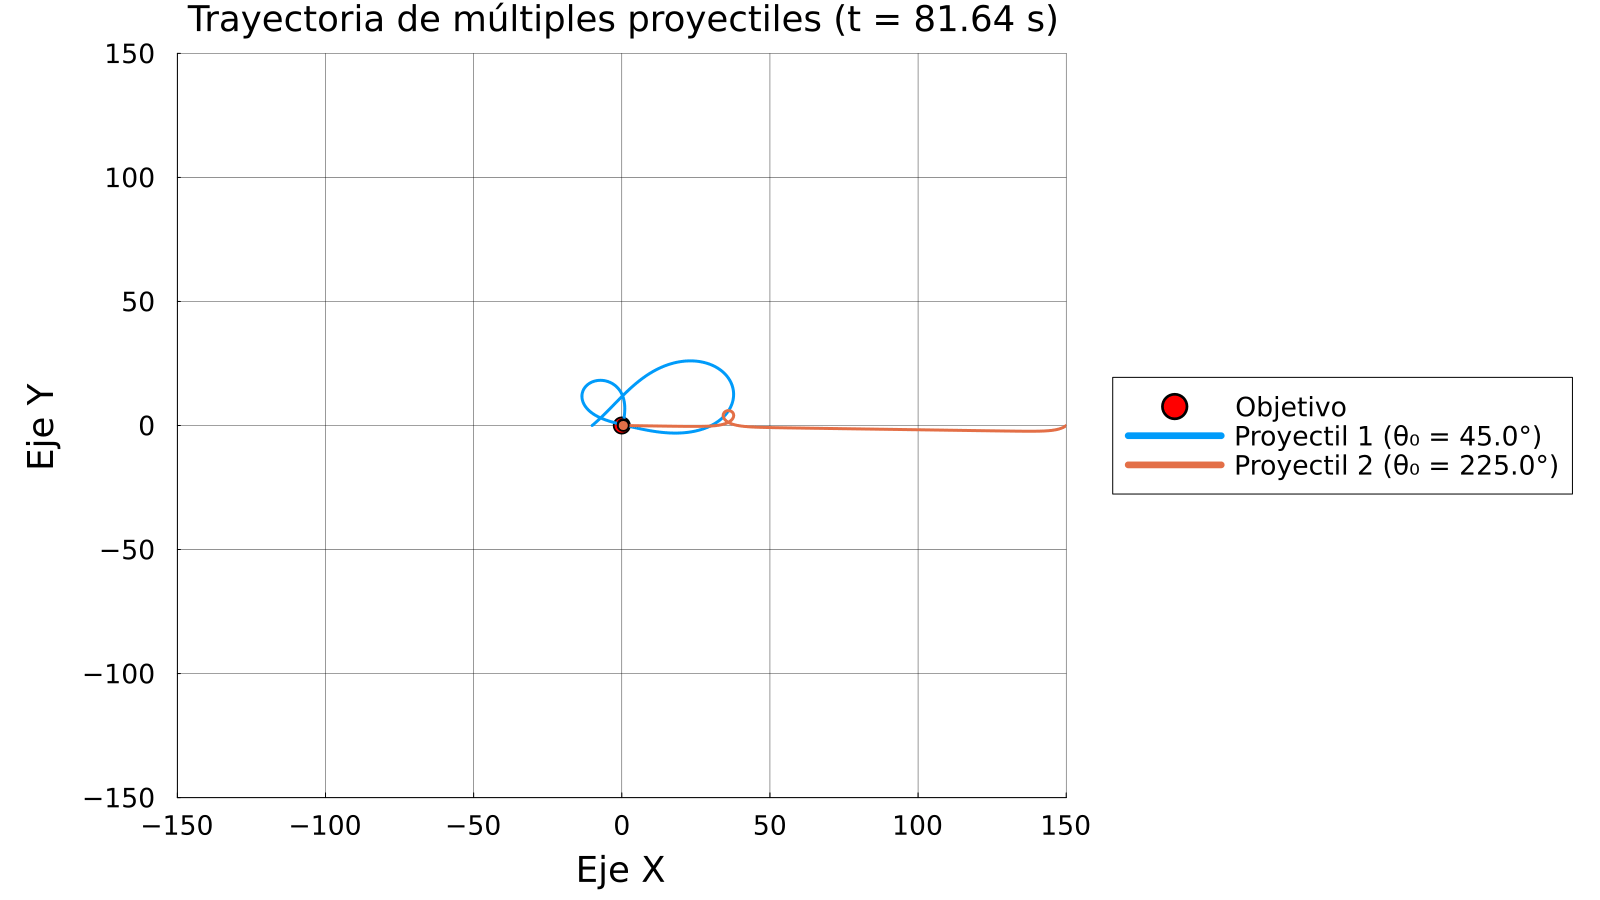
\includegraphics[width=\linewidth]{multiproyectil/posiciones_lejanas_gamma_100.0_final.png}
  \caption{Último fotograma de la animación guardada con $\gamma=100$. \href{run:figuras/multiproyectil/posiciones_lejanas_gamma_100.0.gif}{Animación original}.}
  \label{fig:multi-lejanas-alta}
\end{figure}

\begin{figure}[H]
  \centering
  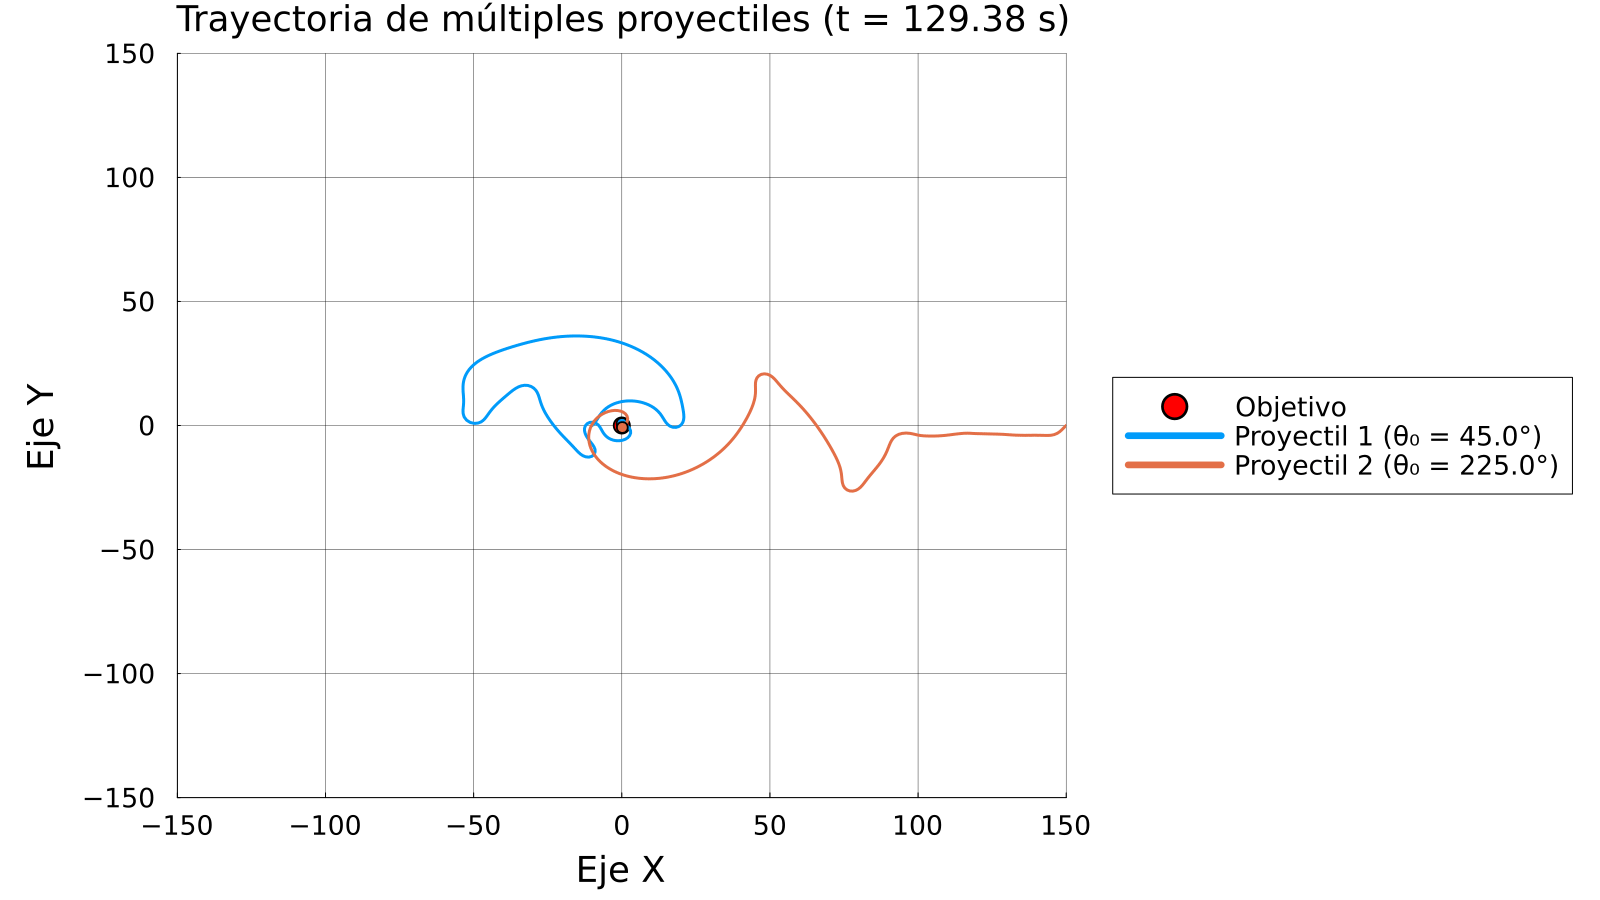
\includegraphics[width=\linewidth]{multiproyectil/posiciones_lejanas_gamma_0.0001_final.png}
  \caption{Último fotograma de la animación guardada con $\gamma=0.0001$. \href{run:figuras/multiproyectil/posiciones_lejanas_gamma_0.0001.gif}{Animación original}.}
  \label{fig:multi-lejanas-baja}
\end{figure}
